\documentclass[10pt]{beamer}
\usetheme[
%%% options passed to the outer theme
%    hidetitle,           % hide the (short) title in the sidebar
%    hideauthor,          % hide the (short) author in the sidebar
%    hideinstitute,       % hide the (short) institute in the bottom of the sidebar
%    shownavsym,          % show the navigation symbols
%    width=2cm,           % width of the sidebar (default is 2 cm)
    hideothersubsections,% hide all subsections but the subsections in the current section
%    hideallsubsections,  % hide all subsections
    left               % right of left position of sidebar (default is right)
%%% options passed to the color theme
%    lightheaderbg,       % use a light header background
  ]{AAUsidebar}

% If you want to change the colors of the various elements in the theme, edit and uncomment the following lines
% Change the bar and sidebar colors:
%\setbeamercolor{AAUsidebar}{fg=red!20,bg=red}
%\setbeamercolor{sidebar}{bg=red!20}
% Change the color of the structural elements:
%\setbeamercolor{structure}{fg=red}
% Change the frame title text color:
%\setbeamercolor{frametitle}{fg=blue}
% Change the normal text color background:
%\setbeamercolor{normal text}{bg=gray!10}
% ... and you can of course change a lot more - see the beamer user manual.


\usepackage[utf8]{inputenc}
\usepackage[english]{babel}
\usepackage[T1]{fontenc}
% Or whatever. Note that the encoding and the font should match. If T1
% does not look nice, try deleting the line with the fontenc.
\usepackage{helvet}

% colored hyperlinks
\newcommand{\chref}[2]{%
  \href{#1}{{\usebeamercolor[bg]{AAUsidebar}#2}}%
}

\title[Autonomous Lawn Mower]% optional, use only with long paper titles
{Autonomous Lawn Mower}

%\subtitle{v.\ 1.4.0}  % could also be a conference name

\date{January 28, 2016}

\author[] % optional, use only with lots of authors
{
	Amalie V. Petersen\\
    Julien Bréhin\\
    Mads R. Gotthardsen\\
    Niels Skov Vestergaard\\
    Romaric Destremau\\
    Thomas Rasmussen
%  Jesper Kjær Nielsen\\
%  \href{mailto:jkn@es.aau.dk}{{\tt jkn@es.aau.dk}}
}
% - Give the names in the same order as they appear in the paper.
% - Use the \inst{?} command only if the authors have different
%   affiliation. See the beamer manual for an example

\institute[
%  {\includegraphics[scale=0.2]{aau_segl}}\\ %insert a company, department or university logo
  SICT\\
  Aalborg University\\
  Denmark
] % optional - is placed in the bottom of the sidebar on every slide
{% is placed on the title page
  SICT\\
  Aalborg University\\
  Denmark
  
  %there must be an empty line above this line - otherwise some unwanted space is added between the university and the country (I do not know why;( )
}


% specify a logo on the titlepage (you can specify additional logos an include them in 
% institute command below
\pgfdeclareimage[height=1.5cm]{titlepagelogo}{AAUgraphics/aau_logo_new} % placed on the title page
%\pgfdeclareimage[height=1.5cm]{titlepagelogo2}{graphics/aau_logo_new} % placed on the title page
\titlegraphic{% is placed on the bottom of the title page
  \pgfuseimage{titlepagelogo}
%  \hspace{1cm}\pgfuseimage{titlepagelogo2}
}


\begin{document}
% the titlepage
{\aauwavesbg%
\begin{frame}[plain,noframenumbering] % the plain option removes the sidebar and header from the title page
  \titlepage
\end{frame}}
%%%%%%%%%%%%%%%%

% TOC
\begin{frame}{Agenda}{}
\setcounter{tocdepth}{1}
\tableofcontents
\end{frame}
%%%%%%%%%%%%%%%%


%%%%%%%%%%%%%%%%%%%%%%%%%%%%%%%%%% NAME %%%%%%%%%%%%%%%%%%%%%%%%%%%%%
%%%%%%%%%%%%%%%%%
\section{Introduction}
%%%%%%%%%%%%%%%%%
%%%%%%%%%%%%%%%%
\subsection{Robotic Lawn mowers}

\begin{frame}{Introduction}{Robotic Lawn mowers}
  \begin{figure}
    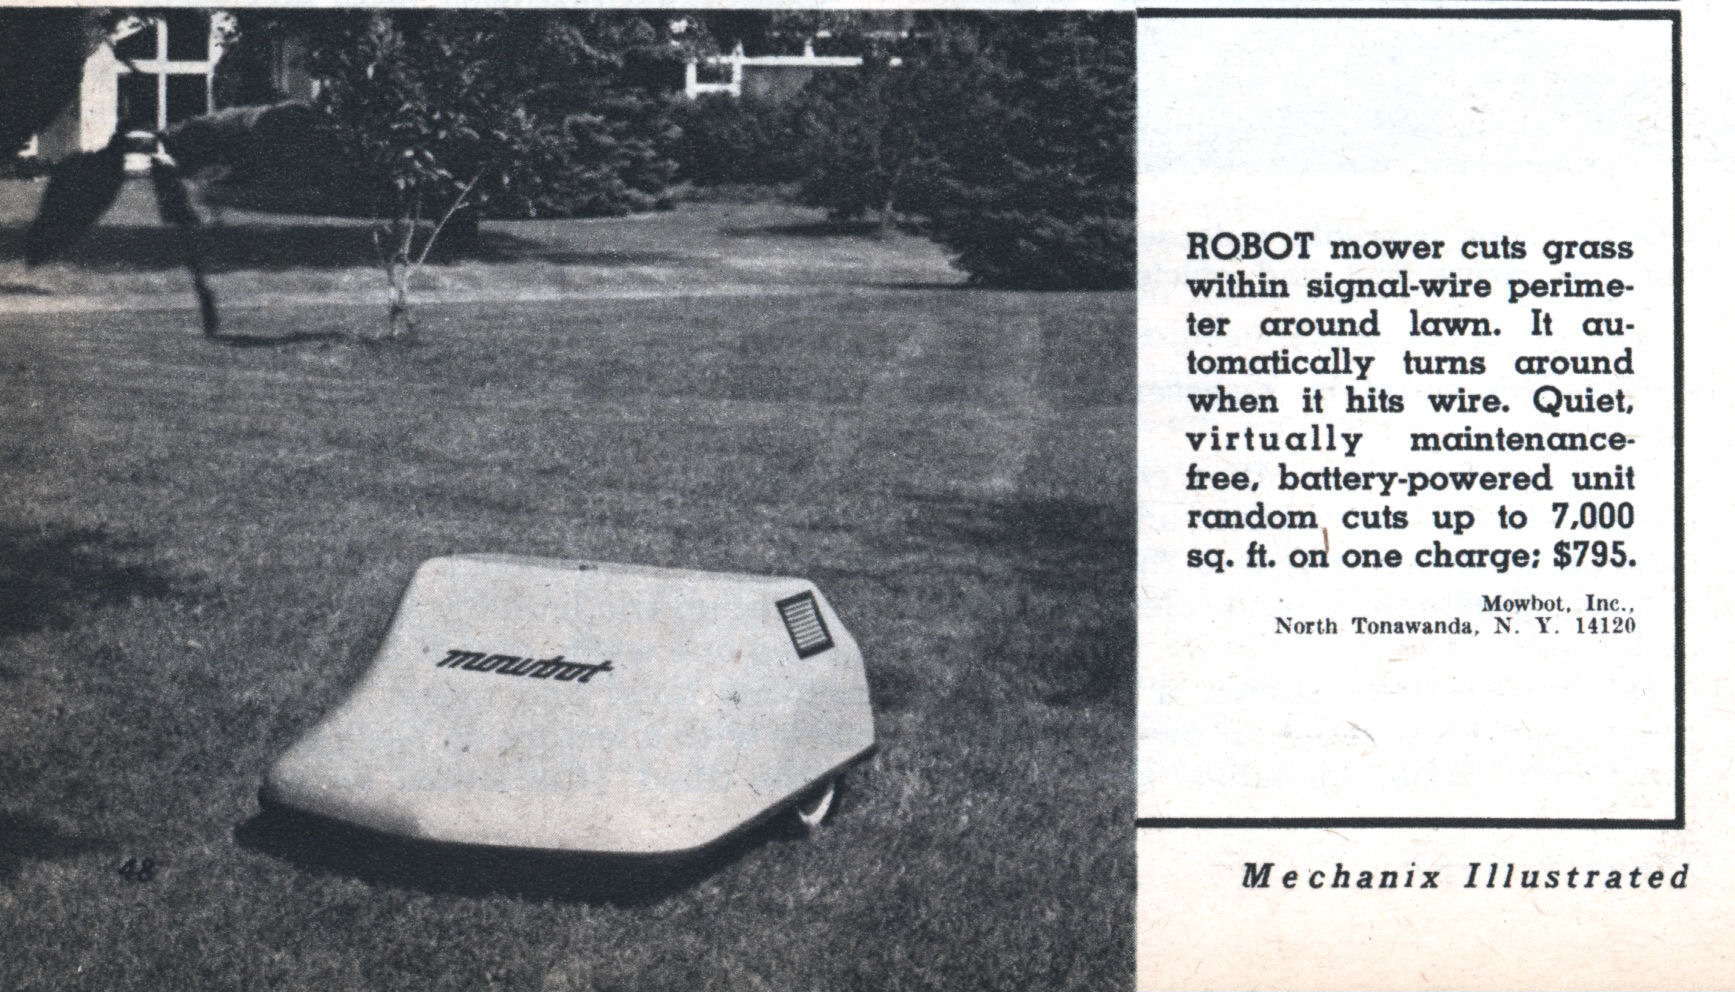
\includegraphics[width=\linewidth]{Pictures/mowbot.jpg}
  \end{figure}
\pause
$$\$795 (1969) \approx \$5296 (2016)$$
\end{frame}
%%%%%%%%%%%%%%%%

%%%%%%%%%%%%%%%%
\subsection{Navigation}

\begin{frame}{Introduction}{Navigation}
    \begin{figure}[!htb]
    \centering
    \begin{minipage}{.8\textwidth}
        \centering
        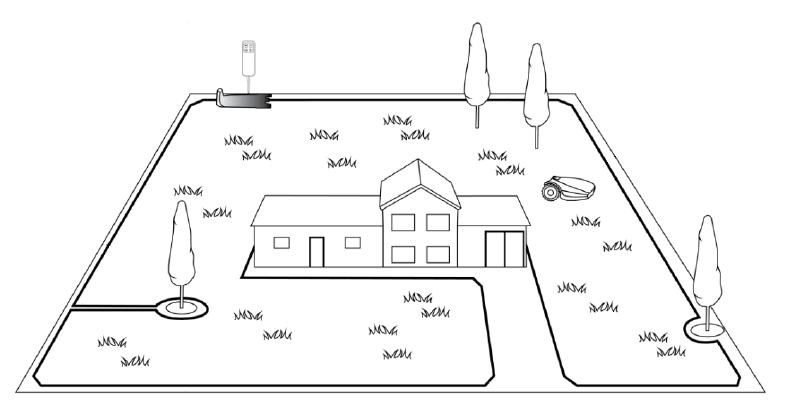
\includegraphics[width=0.99\linewidth]{Pictures/robomow.png}
    \end{minipage}%
    \begin{minipage}{0.2\textwidth}
        \centering
        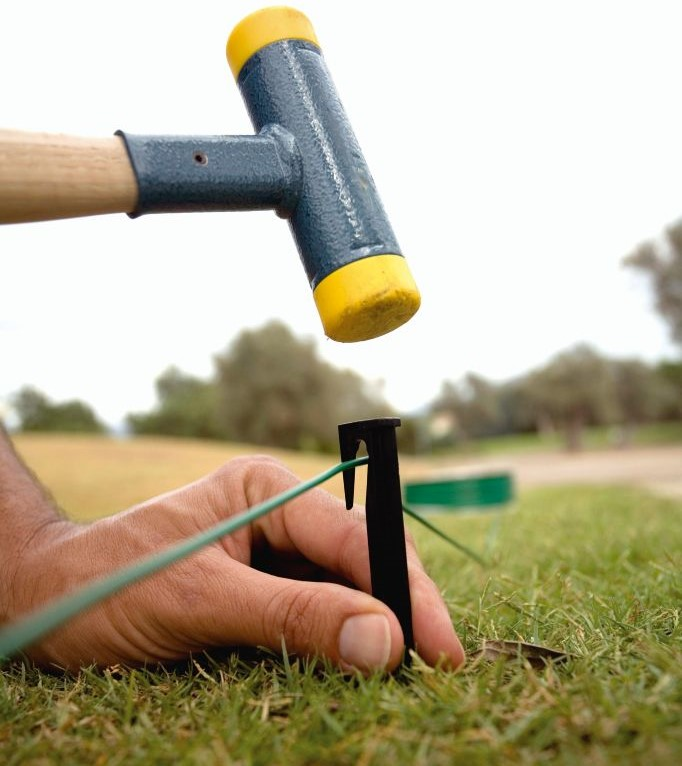
\includegraphics[width=0.99\linewidth]{Pictures/wirehammer.jpg}
    \end{minipage}  
    \end{figure}
\end{frame}
\begin{frame}{Introduction}{Navigation}
    \begin{figure}[!htb]
    \centering
        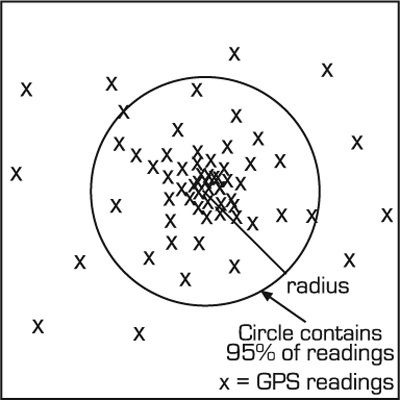
\includegraphics[width=0.7\linewidth]{Pictures/gps.jpg}
    \end{figure}
\end{frame}

%%%%%%%%%%%%%%%%

%%%%%%%%%%%%%%%%
\subsection{Cutting strategies}

\begin{frame}{Introduction}{Cutting strategies}
  Two main types:
 

  \begin{figure}[!htb]
    \centering
    \begin{minipage}{.5\textwidth}
        \centering
        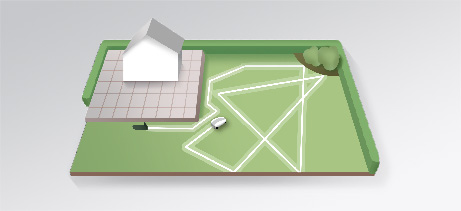
\includegraphics[width=0.99\linewidth]{Pictures/noLogiCut.jpg}
    \end{minipage}%
    \begin{minipage}{0.5\textwidth}
        \centering
        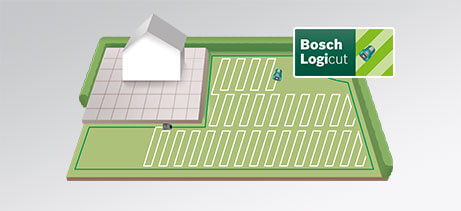
\includegraphics[width=0.99\linewidth]{Pictures/logicut.jpg}
    \end{minipage}
\end{figure}
\vspace{-20pt}
  \begin{table}
   \begin{tabular*}{\columnwidth}{@{\extracolsep{38pt}}cc}
  1. Random direction & 2. Parallel line \\ 
  \end{tabular*} 
\end{table} 

\end{frame}
%%%%%%%%%%%%%%%%


%%%%%%%%%%%%%%%%%%%%%%%%%%%%%%%%%% NAME %%%%%%%%%%%%%%%%%%%%%%%%%%%%%
%%%%%%%%%%%%%%%%%
\section{Design Considerations}
%%%%%%%%%%%%%%%%%

%%%%%%%%%%%%%%%%
\subsection{Use-case Design}

\begin{frame}{Design Considerations}{Use-case Design}
\begin{figure}
\centering
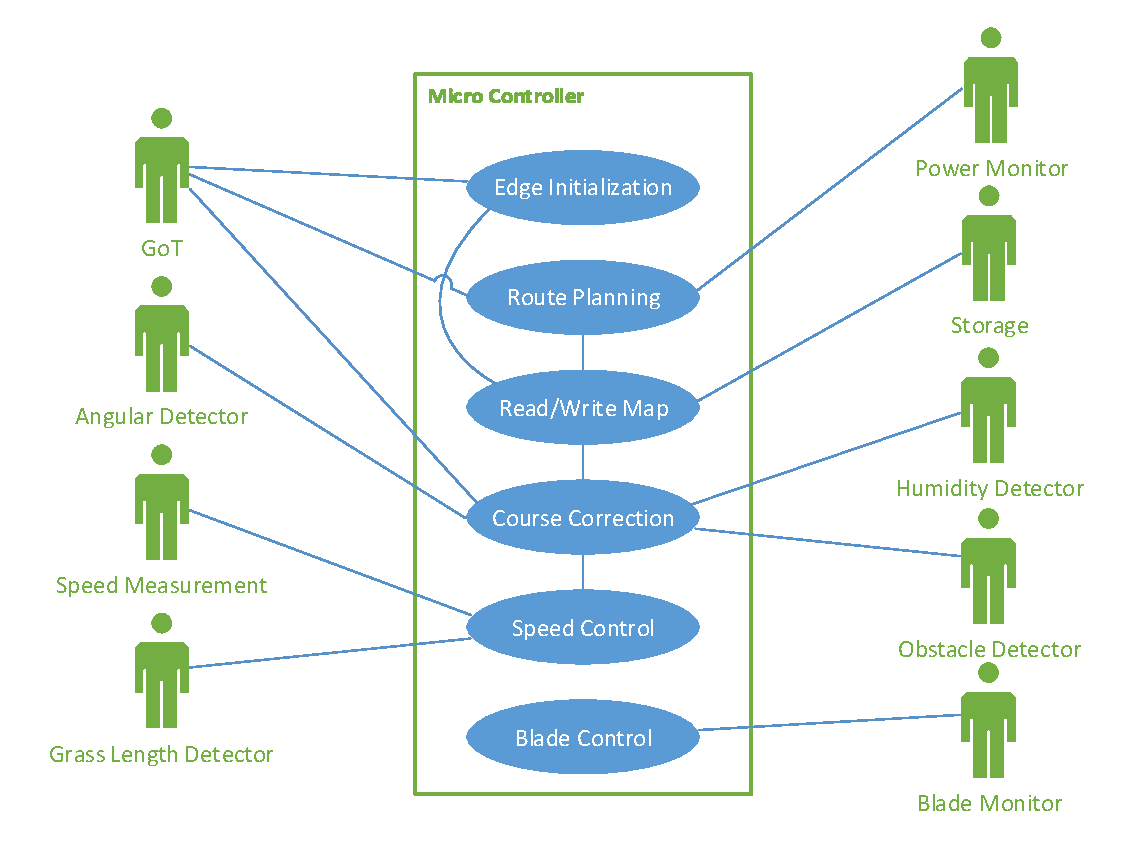
\includegraphics[width=\linewidth]{Pictures/P5UseCase.pdf}
\end{figure}
\end{frame}
%%%%%%%%%%%%%%%%

%%%%%%%%%%%%%%%%
\subsection{Prototype Vehicle}

\begin{frame}{Design Considerations}{Prototype Vehicle}
\begin{figure}
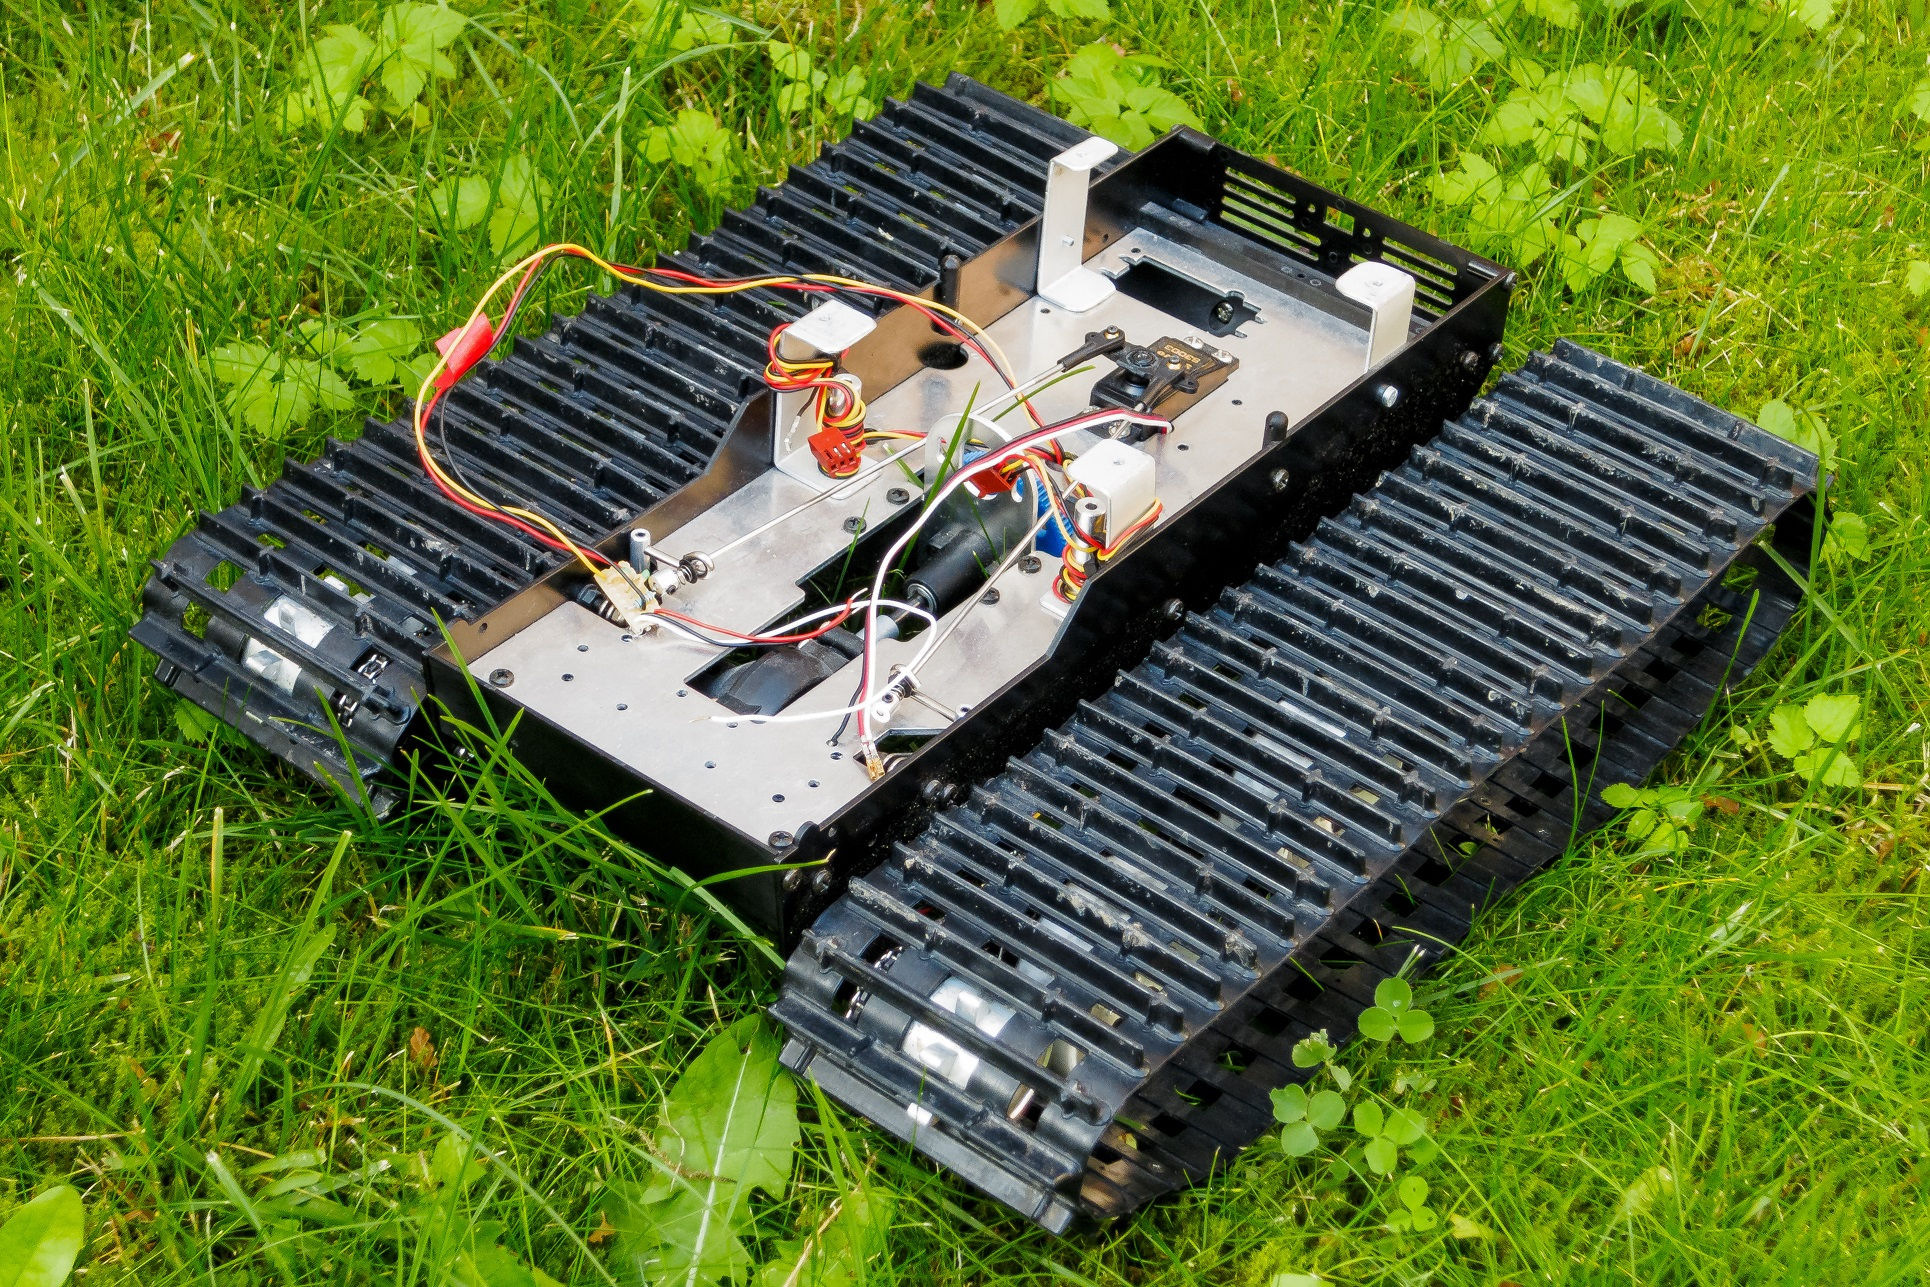
\includegraphics[width=\textwidth]{Pictures/BeltVehicle.jpg}
\end{figure}
\end{frame}
\begin{frame}{Design Considerations}{Prototype Vehicle}
\begin{figure}
\includegraphics[width=\textwidth]{Pictures/FullVehicle.png}
\end{figure}
\end{frame}


\section{Prototype Requirements}
\begin{frame}{Prototype Requirements}
\begin{figure}
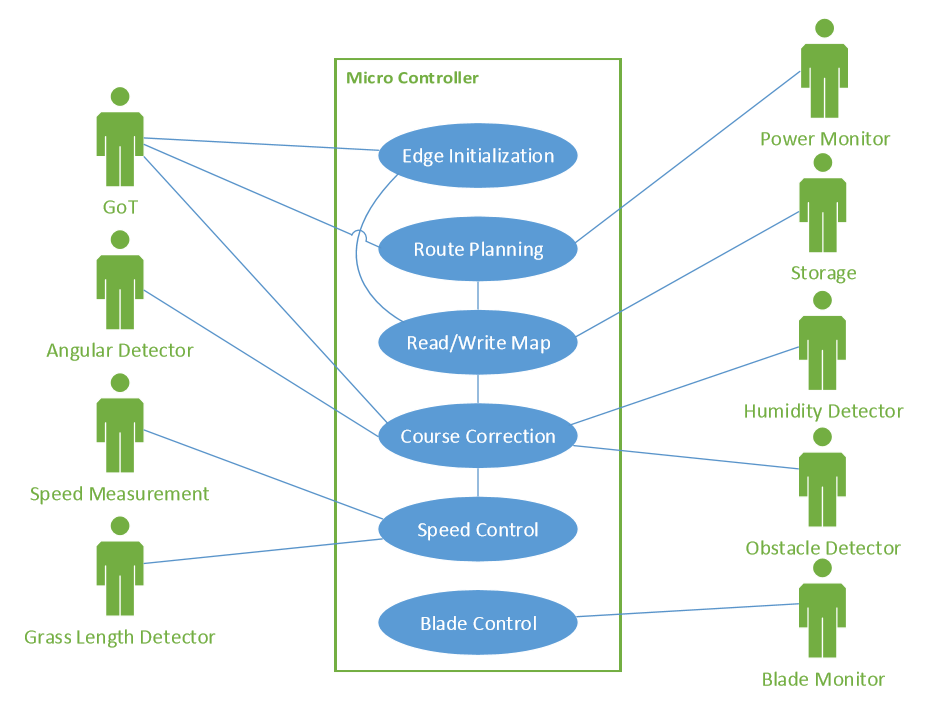
\includegraphics[width=\textwidth]{Pictures/uc1.png}
\end{figure}
\end{frame}
\begin{frame}{Prototype Requirements}
\begin{figure}
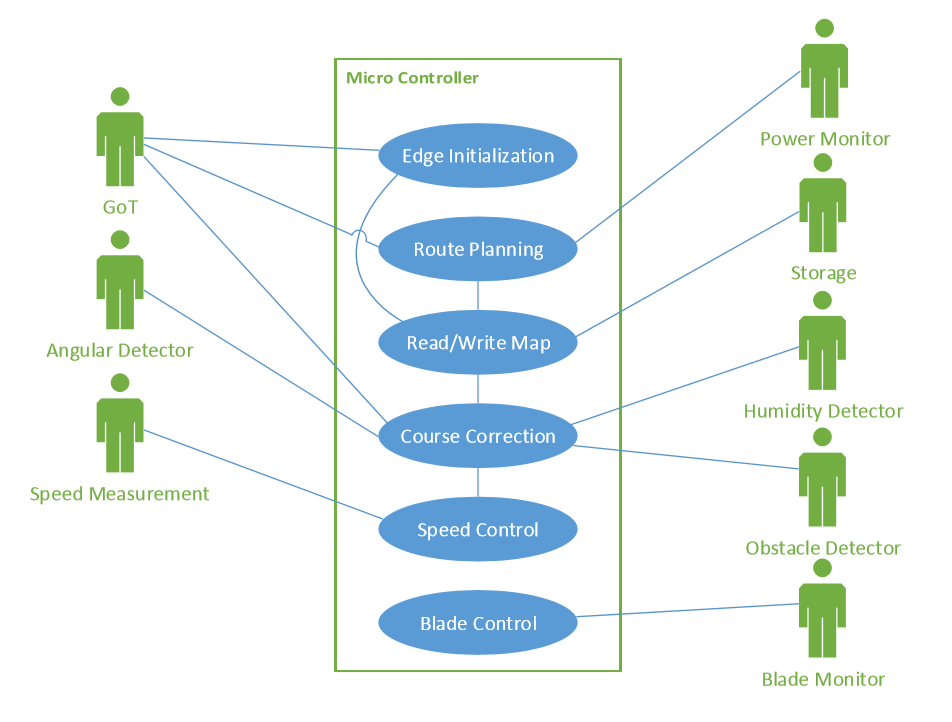
\includegraphics[width=\textwidth]{Pictures/uc2.png}
\end{figure}
\end{frame}
\begin{frame}{Prototype Requirements}
\begin{figure}
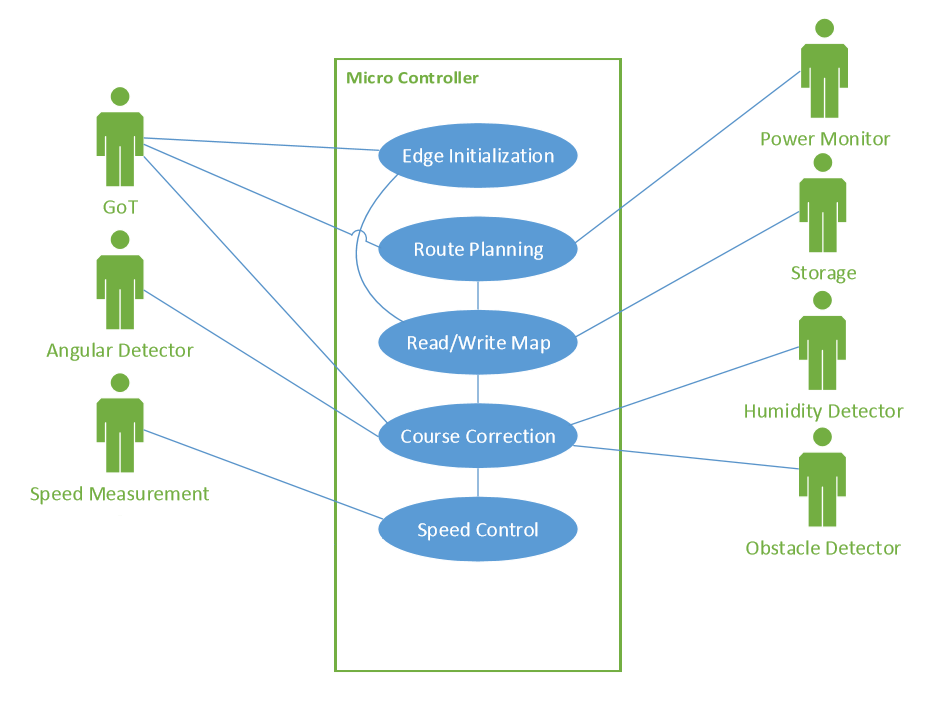
\includegraphics[width=\textwidth]{Pictures/uc3.png}
\end{figure}
\end{frame}
\begin{frame}{Prototype Requirements}
\begin{figure}
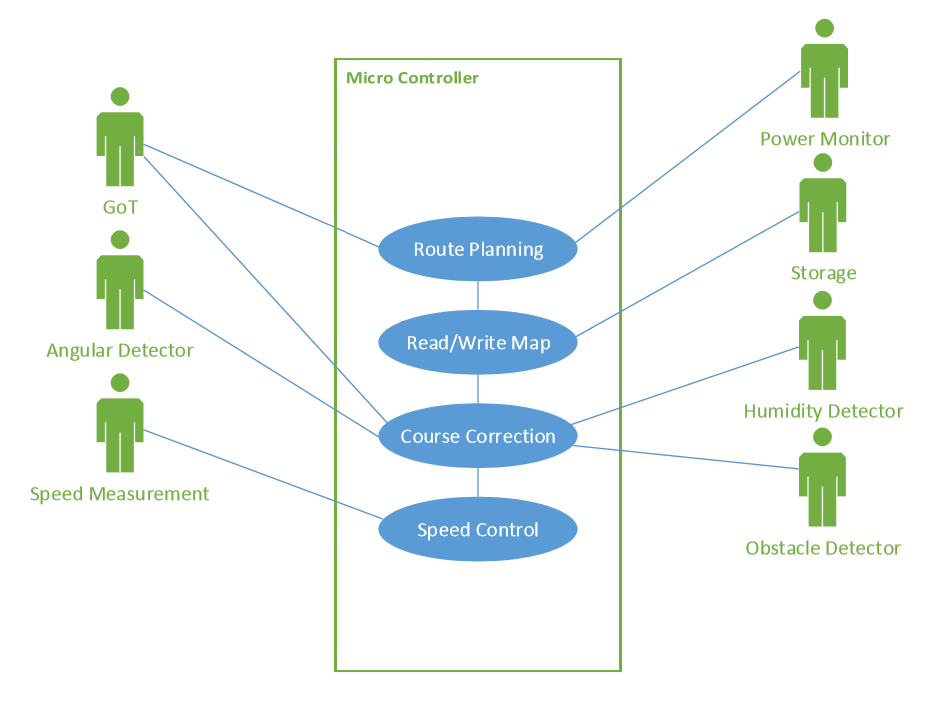
\includegraphics[width=\textwidth]{Pictures/uc4.png}
\end{figure}
\end{frame}
\begin{frame}{Prototype Requirements}
\begin{figure}
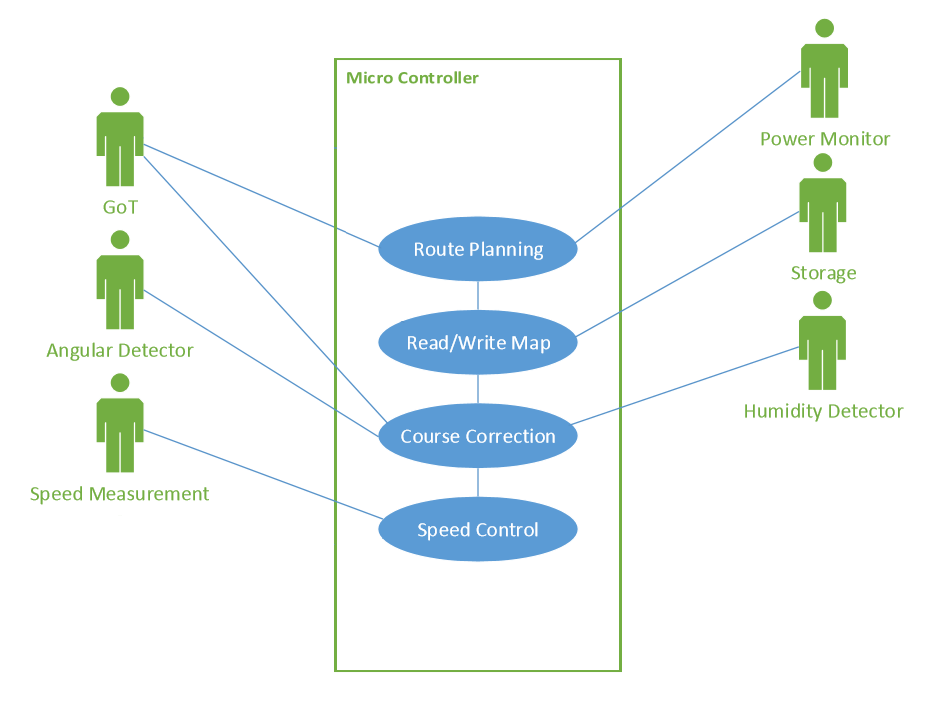
\includegraphics[width=\textwidth]{Pictures/uc5.png}
\end{figure}
\end{frame}
\begin{frame}{Prototype Requirements}
\begin{figure}
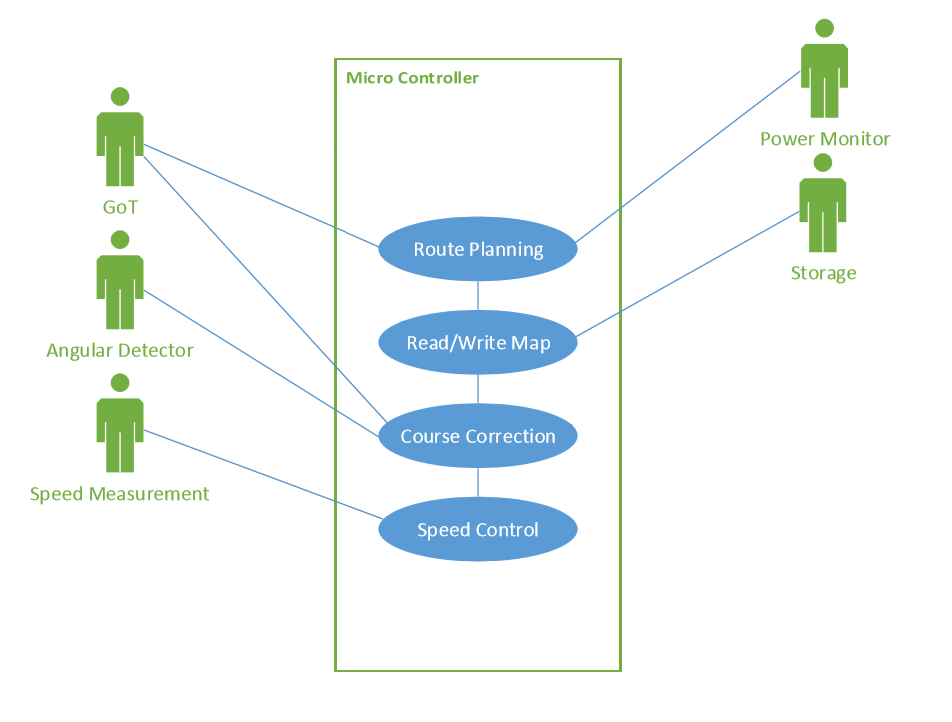
\includegraphics[width=\textwidth]{Pictures/uc6.png}
\end{figure}
\end{frame}
%%%%%%%%%%%%%%%%
%%%%%%%%%%%%%%%%%%%%%%%%%%%%%%%%%% NAME %%%%%%%%%%%%%%%%%%%%%%%%%%%%%
%%%%%%%%%%%%%%%%%


\begin{frame}{Prototype Requirements}
  \begin{enumerate}
\footnotesize
\item \textbf{It shall be possible for the vehicle to receive its own location wirelessly from the GoT system, through a computer.}
\item \textbf{It shall be possible for the prototype to disregard incorrect packets transmitted from the computer}
	\item \textbf{The prototype must be able to disregard erroneous coordinates sent from the GoT system}
\item \textbf{The prototype must be able to access the route, which it has to follow, from a storage space located on the vehicle}
\item \textbf{The prototype must be able to shut down, if the battery voltage is below its cut-off specification}
\item \textbf{It shall be possible for the prototype to follow a predetermined route}
\item \textbf{It shall be possible for the prototype to return to the predetermined route if disturbed}
\item \textbf{The prototype shall be able to keep a velocity on 1,4 $m \cdot s^{-1}$, when going up - or downhill and when turning}
\end{enumerate}
\end{frame}
%%%%%%%%%%%%%%%%%

%%%%%%%%%%%%%%%%%%%%%%%%%%%%%%%%%% NAME %%%%%%%%%%%%%%%%%%%%%%%%%%%%%
%%%%%%%%%%%%%%%%%
\section{Hardware and Software}
%%%%%%%%%%%%%%%%
\subsection{Prototype overview}

\begin{frame}{Hardware and Software}{Prototype overview}
  \begin{figure}[H]
	\centering
	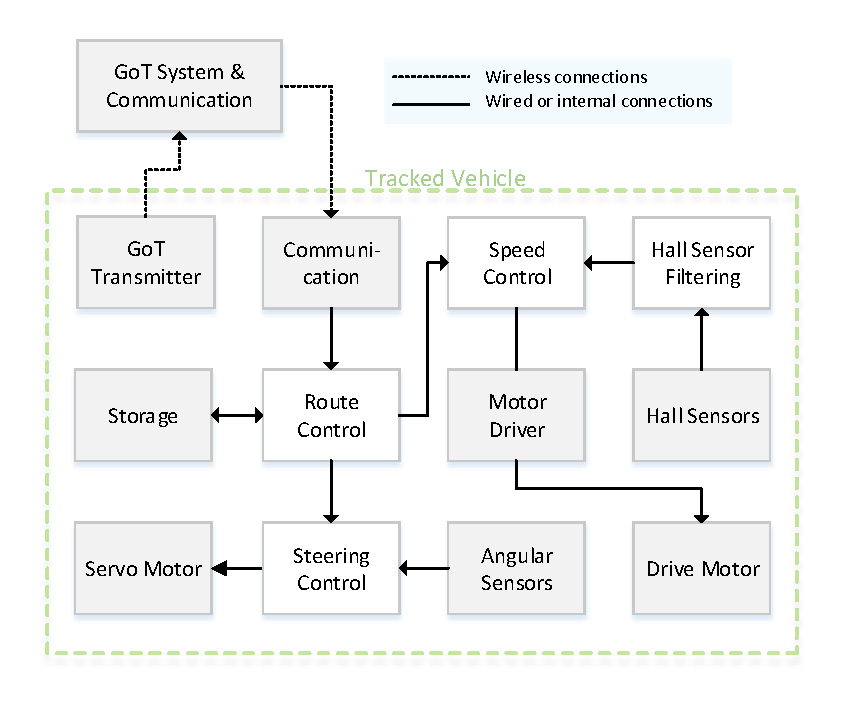
\includegraphics[scale=0.65]{Pictures/SO3.pdf}
  \end{figure}
\end{frame}
%%%%%%%%%%%%%%%%

%%%%%%%%%%%%%%%%
\subsection{Hardware components}

\begin{frame}{Hardware and Software}{Hardware components}
\textbf{Controller}
\begin{itemize}
\item{Arduino Mega 2560}
\end{itemize}
  \begin{figure}[H]
	\centering
	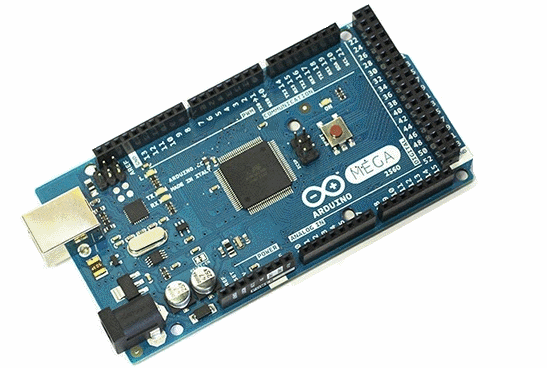
\includegraphics[scale=0.4]{Pictures/ArduinoMega.png}
  \end{figure}
\end{frame}

\begin{frame}{Hardware and Software}{Hardware components}
\textbf{Velocity Sensor}
\begin{itemize}
\item{Hall Sensor}
\end{itemize}
  \begin{figure}[H]
	\centering
	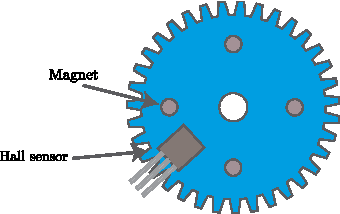
\includegraphics[scale=1.5]{Pictures/hallSensorDrawing.pdf}
  \end{figure}
\end{frame}

\begin{frame}{Hardware and Software}{Hardware components}
\textbf{Angular Sensor}
\begin{itemize}
\item{HMC5883L Magnetometer}
\end{itemize}

  \begin{minipage}{\linewidth}
  	\begin{minipage}{0.45\linewidth}
  		\begin{figure}[H]
  			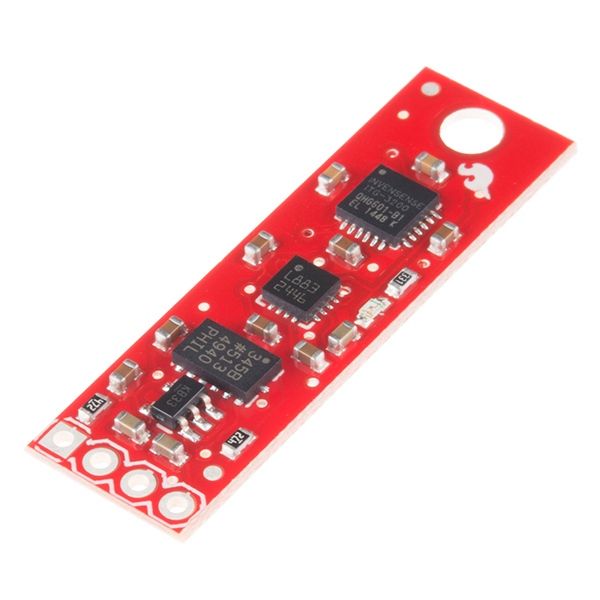
\includegraphics[scale=0.7]{Pictures/NineDegree.jpg}
  			\centering
  		\end{figure}
  	\end{minipage}
  	\hspace{0.03\linewidth}
  	\begin{minipage}{0.45\linewidth}
  		\begin{figure}[H]
  			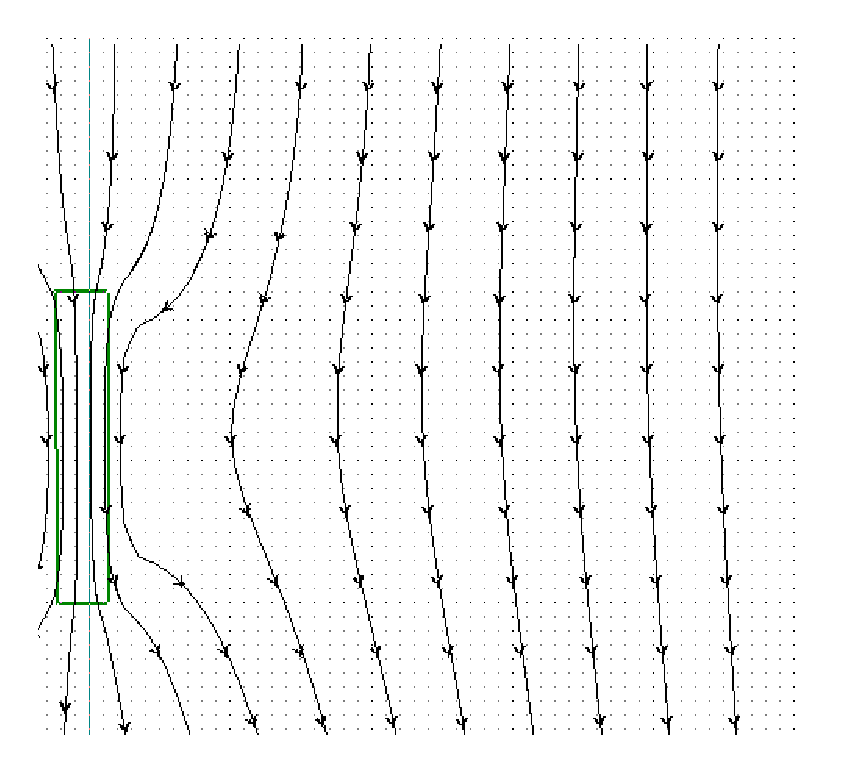
\includegraphics[scale=0.35]{Pictures/Magne.pdf}
  			\centering
  		\end{figure}
  	\end{minipage}
  \end{minipage}

\end{frame}




\begin{frame}{Hardware and Software}{Hardware components}
\textbf{Position Sensor}
\begin{itemize}
\item{Games on Track system (GoT)}
\end{itemize}
  \begin{figure}[H]
	\centering
	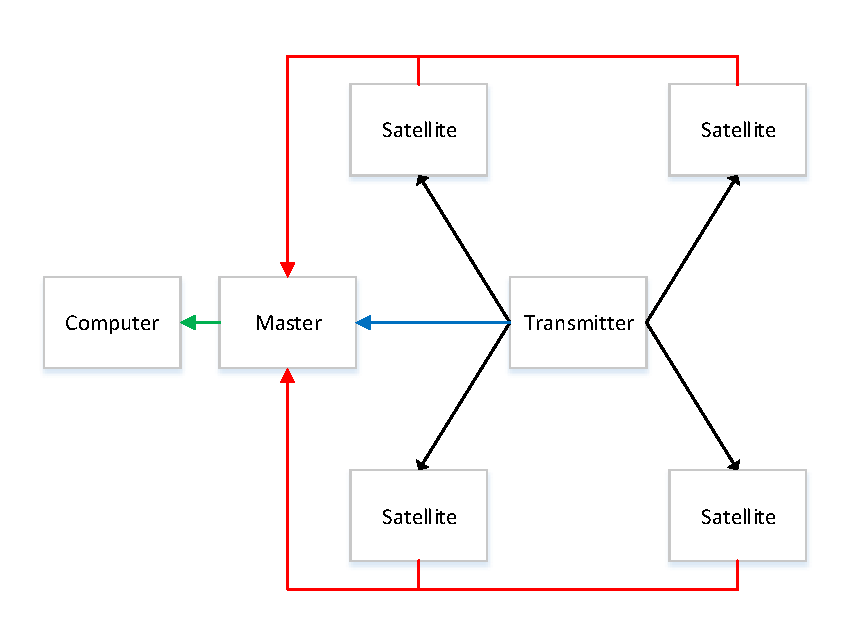
\includegraphics[scale=0.6]{Pictures/GOTNew.pdf}
  \end{figure}
\end{frame}

\begin{frame}{Hardware and Software}{Hardware components}
\begin{itemize}
\item {Communication}
\item {Storage}
\item {Motor driver}
\item {Battery and Power monitor}
\end{itemize}
\end{frame}
%%%%%%%%%%%%%%%%

%%%%%%%%%%%%%%%%
\subsection{Software}

\begin{frame}{Hardware and Software}{Software}
\begin{itemize}
 \item {Real Time Operating System}
  \begin{itemize}
	\item {KRNL by Jens Dalsgaard Nielsen}
\end{itemize}
\end{itemize}

  \begin{figure}[H]
	\centering
	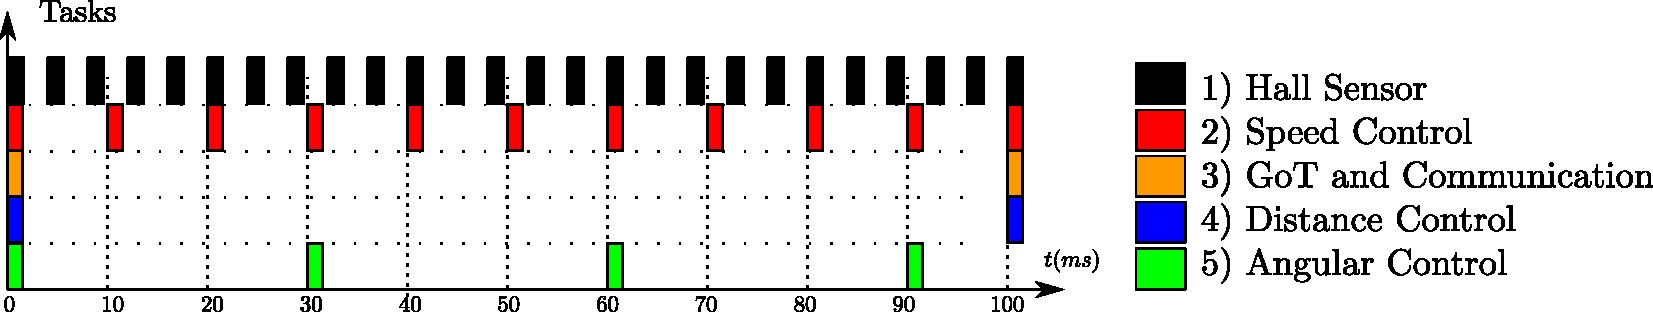
\includegraphics[scale=0.35]{Pictures/scheduleRequest.pdf}
  \end{figure}

  \begin{figure}[H]
	\centering
	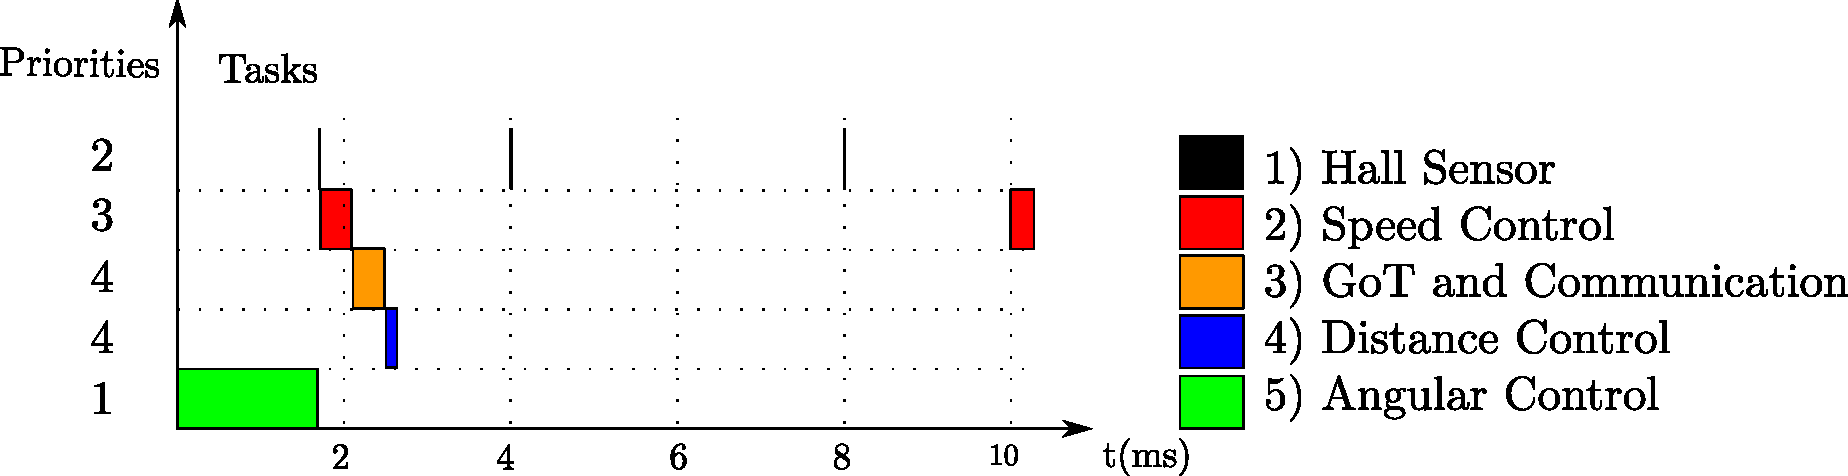
\includegraphics[scale=0.3]{Pictures/schedulePriorities.pdf}
  \end{figure}
\end{frame}
%%%%%%%%%%%%%%%%%%%%%%%%%%%%%%%%%% NAME %%%%%%%%%%%%%%%%%%%%%%%%%%%%%

%%%%%%%%%%%%%%%%%
\section{Modeling of the Vehicle}

\begin{frame}{Modeling of the Vehicle}{}
  
  \begin{figure}[H]
	\centering
	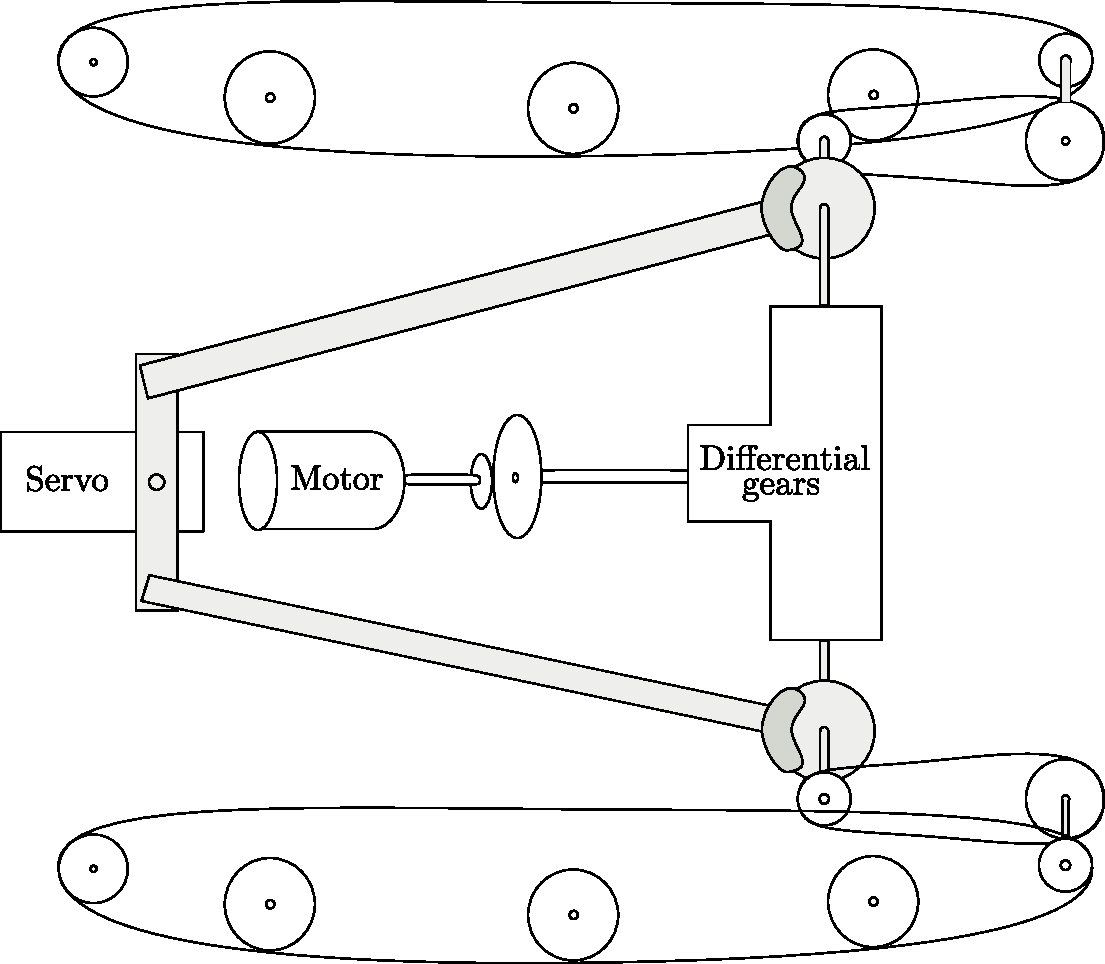
\includegraphics[scale=0.4]{Pictures/completeMechanical.pdf}
\end{figure}
  
\end{frame}
%%%%%%%%%%%%%%%%%

%%%%%%%%%%%%%%%%%
\section{Velocity Model}

\begin{frame}{Velocity Model}{}
  
    \begin{figure}[H]
	\centering
	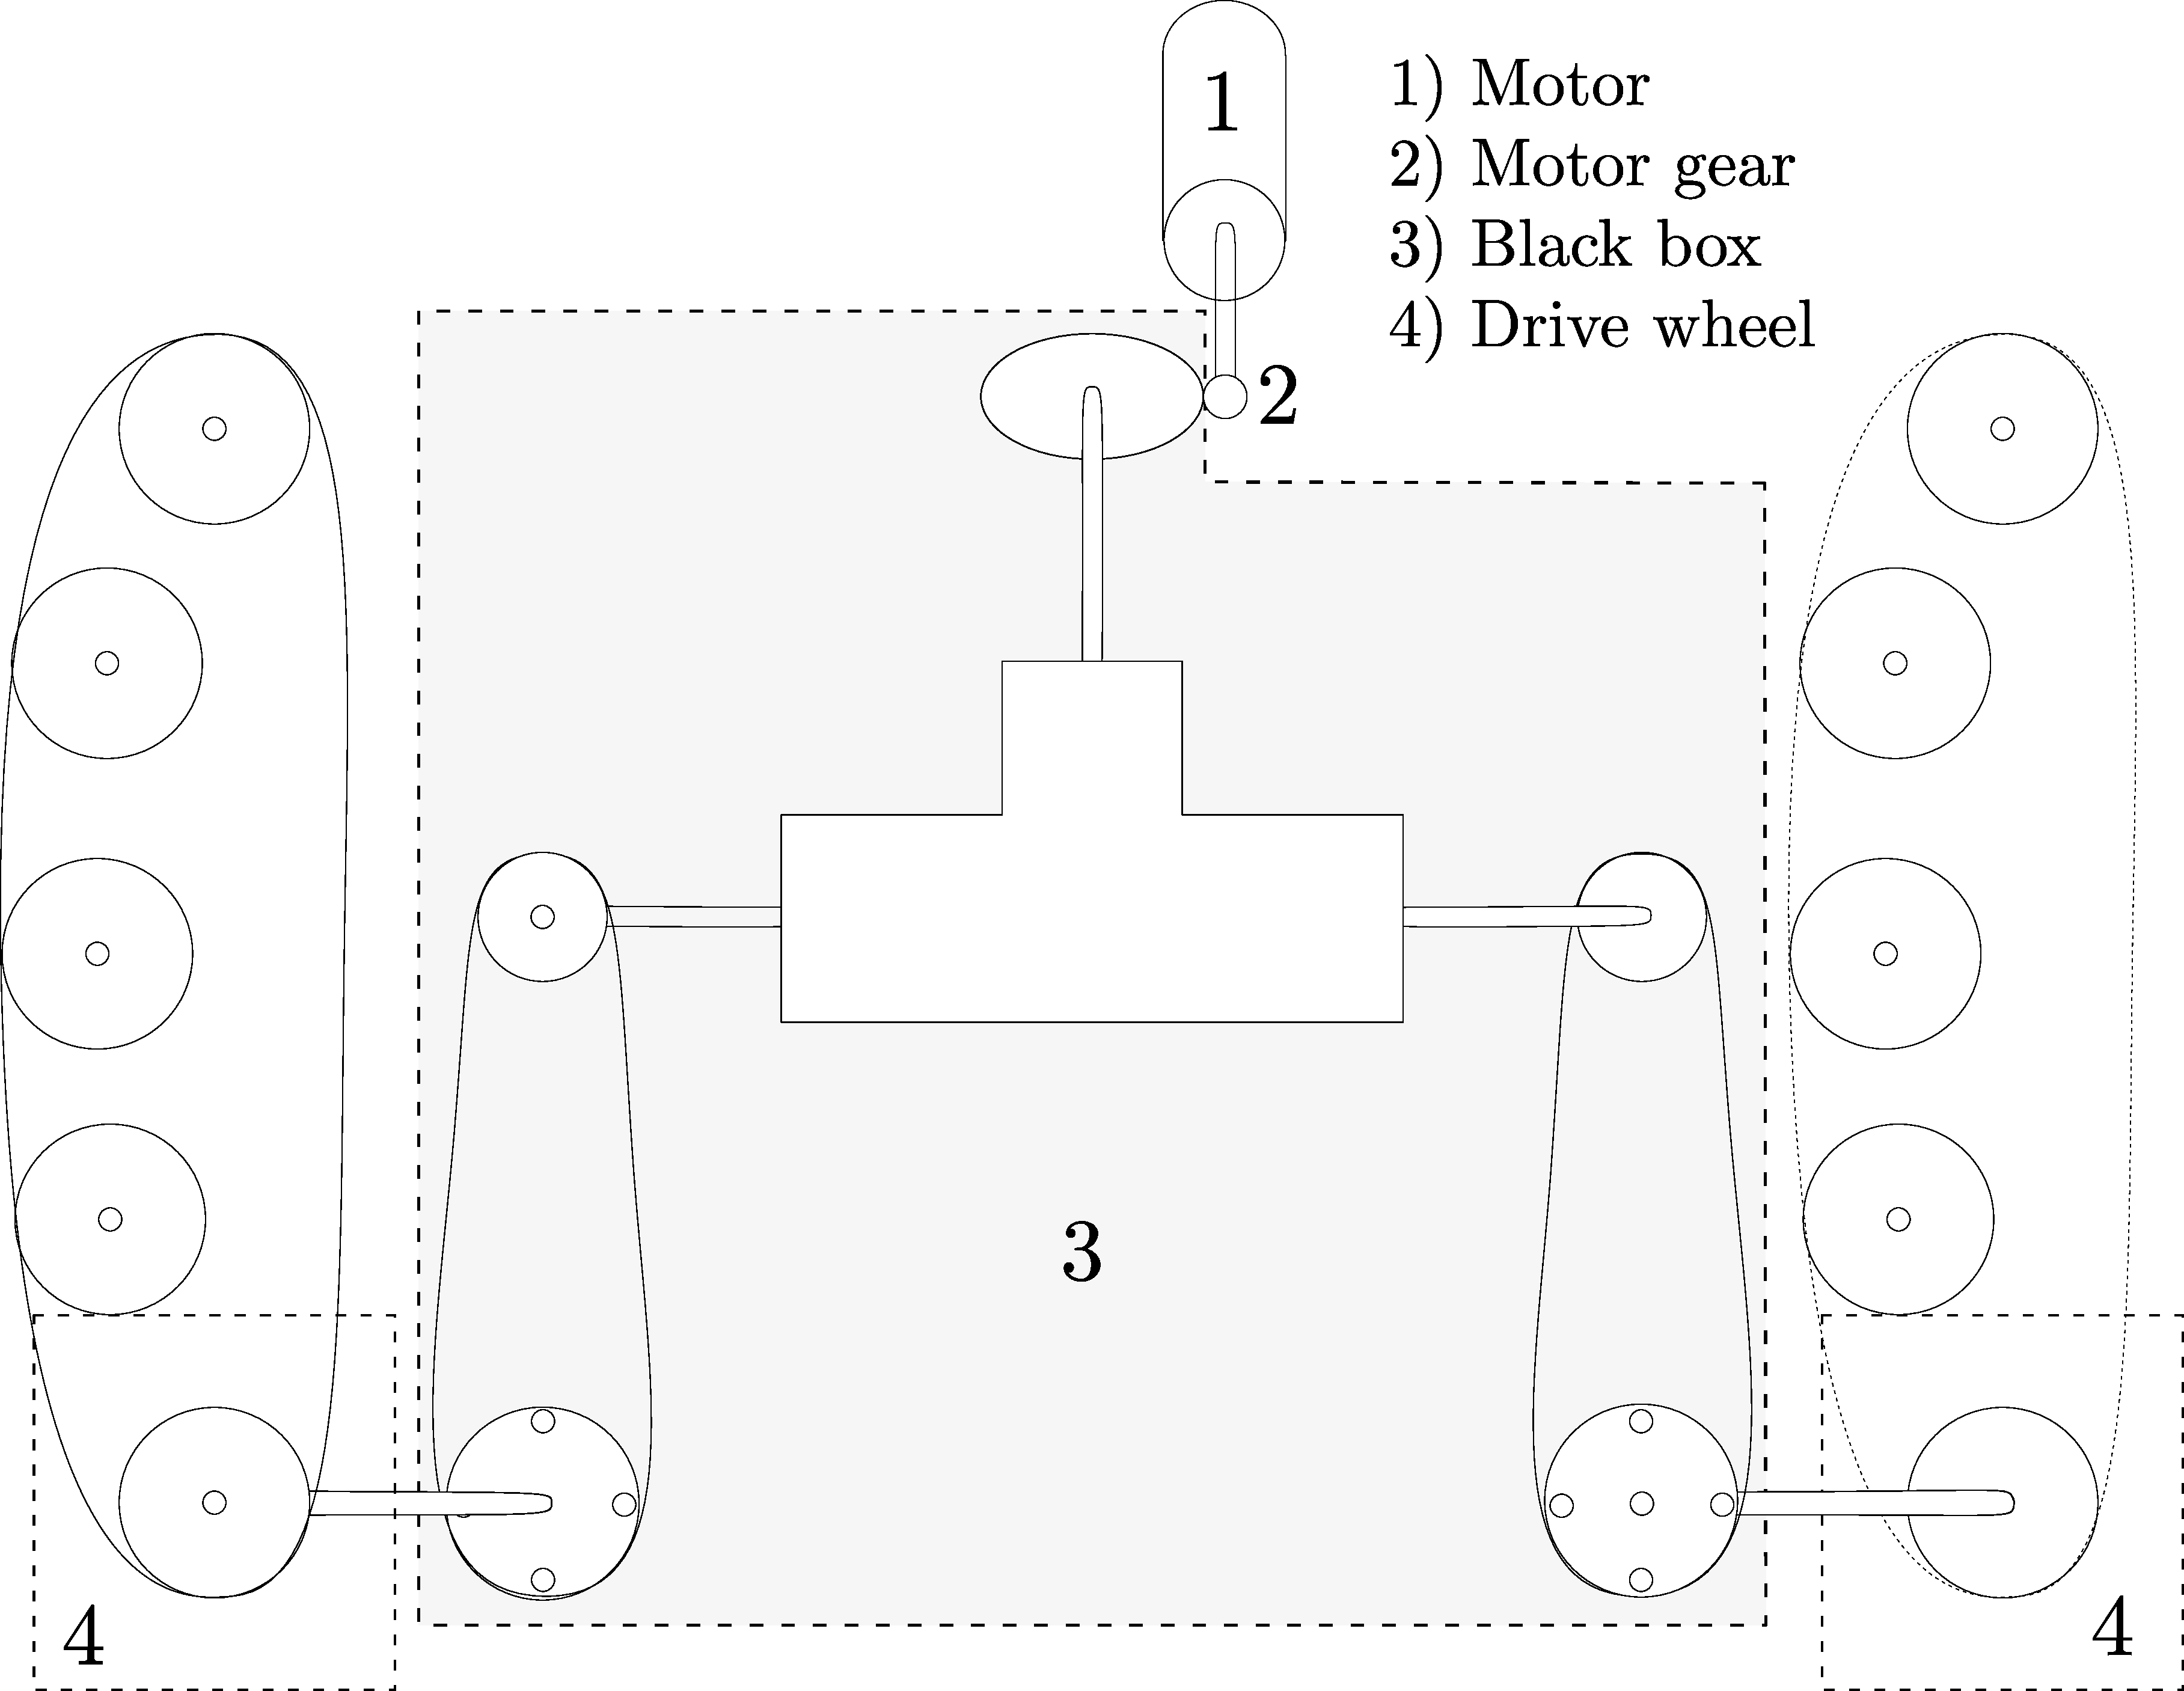
\includegraphics[scale=0.15]{Pictures/vehicleDescriptionDriveTrainBlackBox2.pdf}
    
\end{figure}

\end{frame}
%%%%%%%%%%%%%%%%%

%%%%%%%%%%%%%%%%
%\subsection{Free Body Diagrams}

\begin{frame}{Velocity Model}{Electrical diagram}

\vspace{-10pt}

\begin{figure}[H]
	\centering
	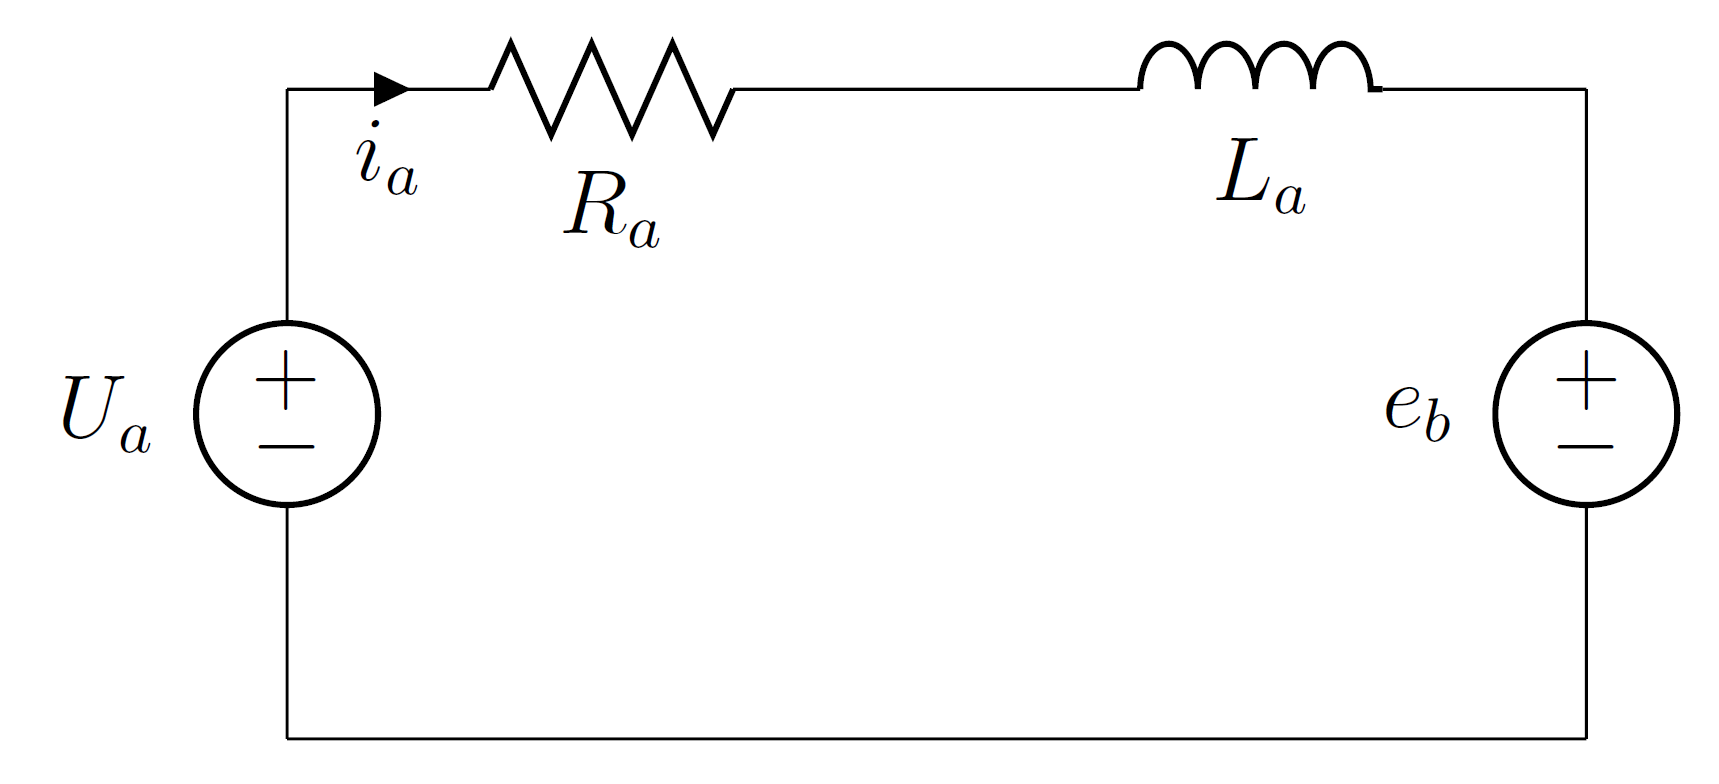
\includegraphics[scale=0.2]{Pictures/ElectricalDiagram.PNG}  
\end{figure}

\begin{figure}[H]
	\centering
	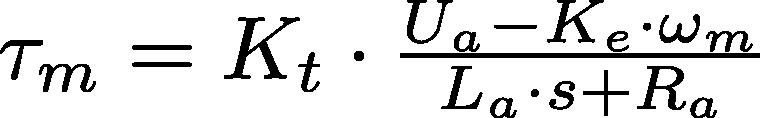
\includegraphics[scale=0.5]{Pictures/ElectricTorqu.pdf}  
\end{figure}

\vspace{20pt}

\end{frame}
%%%%%%%%%%%%%%%%

%%%%%%%%%%%%%%%%
%\subsection{Free Body Diagrams}

\begin{frame}{Velocity Model}{Free body diagram}

\begin{figure}[H]
	\centering
	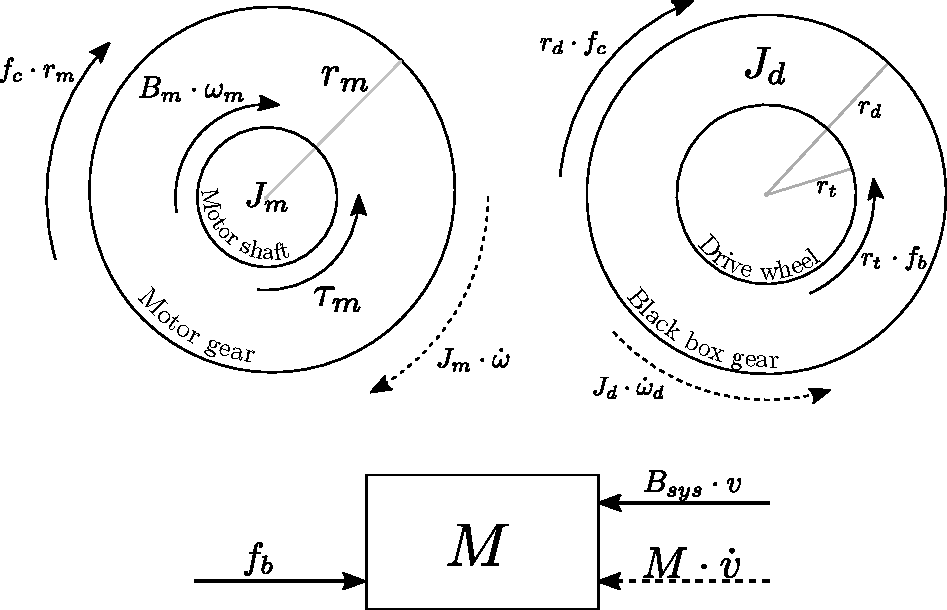
\includegraphics[scale=0.6]{Pictures/freebodydiagramtogether.pdf}
    
\end{figure}

\end{frame}
%%%%%%%%%%%%%%%%

%%%%%%%%%%%%%%%%
\subsection{Final Velocity Model}

\begin{frame}{Velocity Model}{Final Velocity Model}

\vspace{-20pt}

\begin{figure}[H]
	\centering
	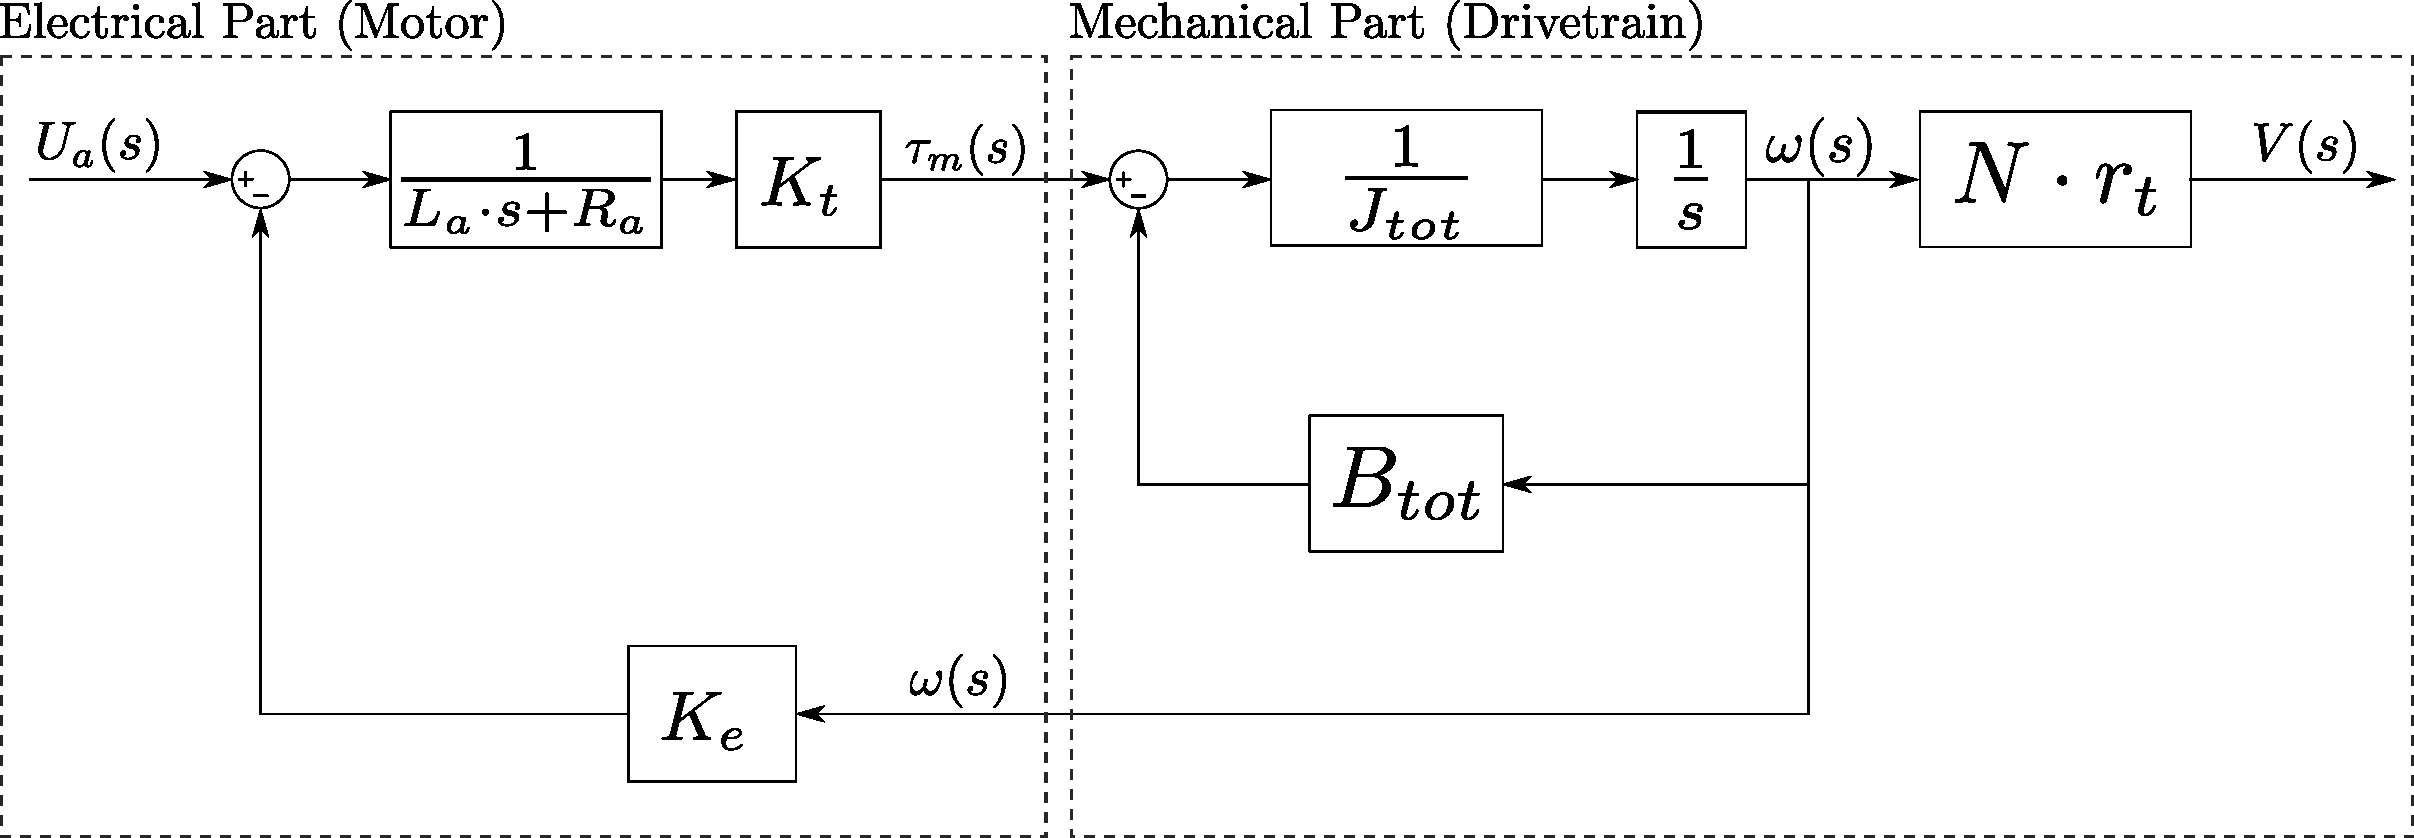
\includegraphics[scale=0.24]{Pictures/totalVelocityModelDiagramNotComplicated.pdf}   
\end{figure}

\vspace{10pt}

    \begin{figure}[H]
	\centering
	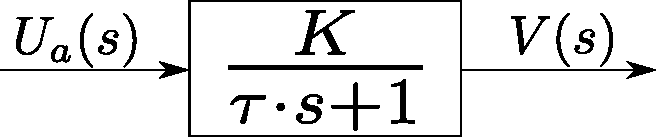
\includegraphics[scale=0.5]{Pictures/totalVelocityModelDiagramSimplified.pdf}
    
\end{figure}

\end{frame}
%%%%%%%%%%%%%%%%

%%%%%%%%%%%%%%%%
\subsection{Verification of the Velocity Model}

\begin{frame}{Velocity Model}{Verification of the Velocity Model}

\begin{figure}[H]
	\centering
	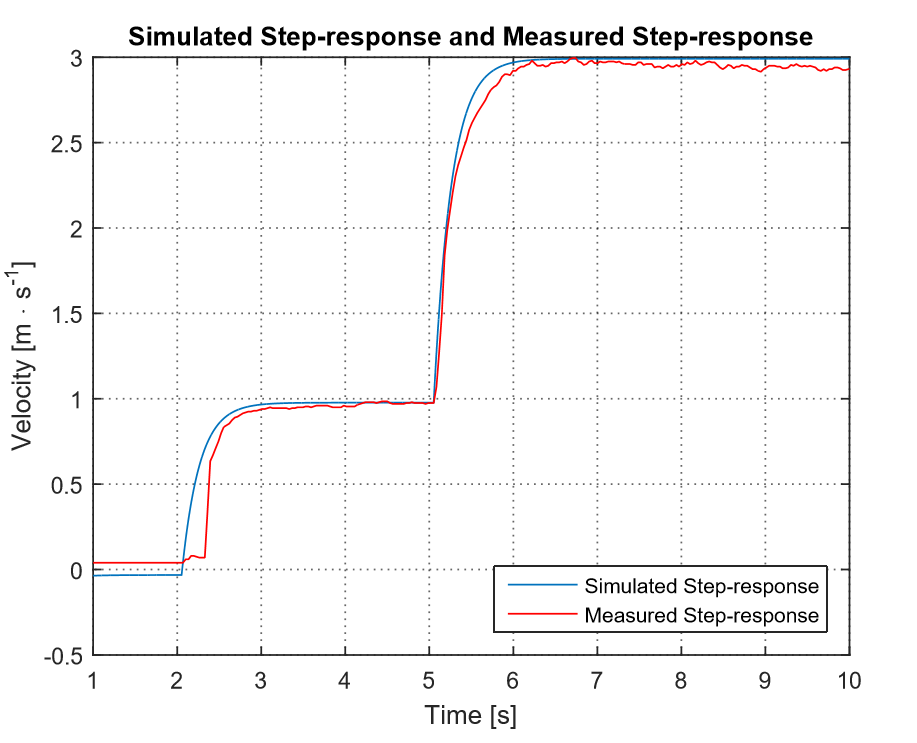
\includegraphics[scale=0.39]{Pictures/amaliehererden.png}   
\end{figure}

\end{frame}
%%%%%%%%%%%%%%%%

%%%%%%%%%%%%%%%%
\section{Velocity Controller}

\begin{frame}{Velocity Controller}{P-Controller and P-Controller with feed forward}

\begin{figure}[H]
	\centering
	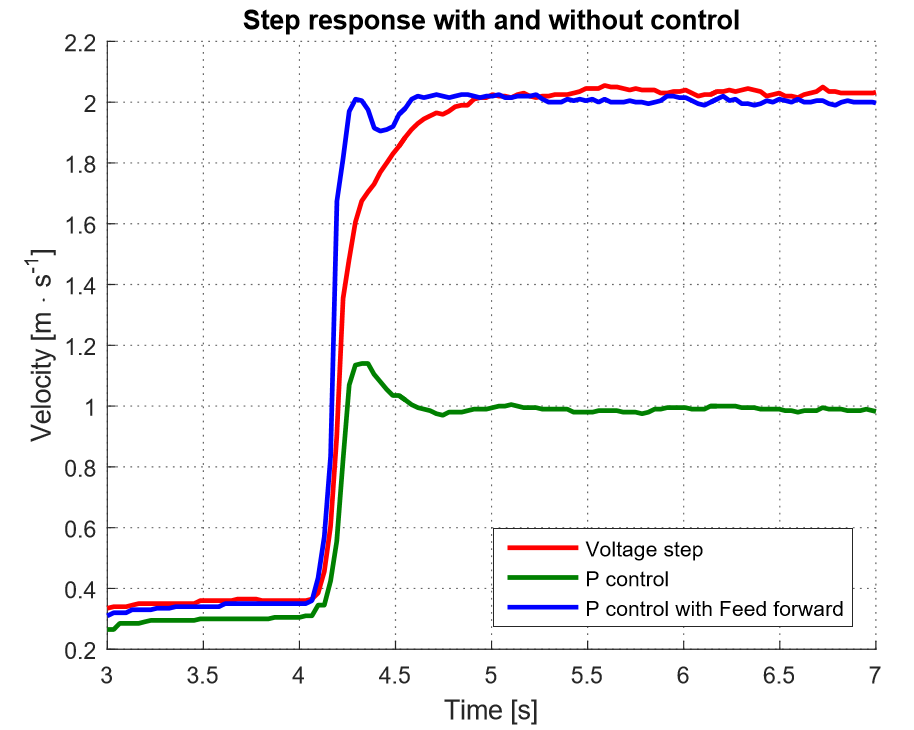
\includegraphics[scale=0.39]{Pictures/stepWithPControl2.png}   
\end{figure}

\end{frame}
%%%%%%%%%%%%%%%%

%%%%%%%%%%%%%%%%
\subsection{P-Controller with Feed Forward}

\begin{frame}{Velocity Controller}{P-Controller with Feed Forward}

\begin{figure}[H]
	\centering
	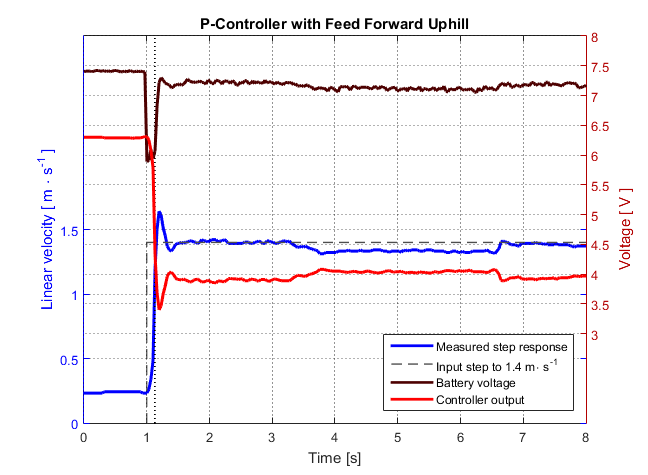
\includegraphics[scale=0.55]{Pictures/hillPfeedForward.png}   
\end{figure}

\end{frame}
%%%%%%%%%%%%%%%%

%%%%%%%%%%%%%%%%
%\subsection{PI-Controller}

\begin{frame}{Velocity Controller}{PI-Controller}

\begin{figure}[H]
	\centering
	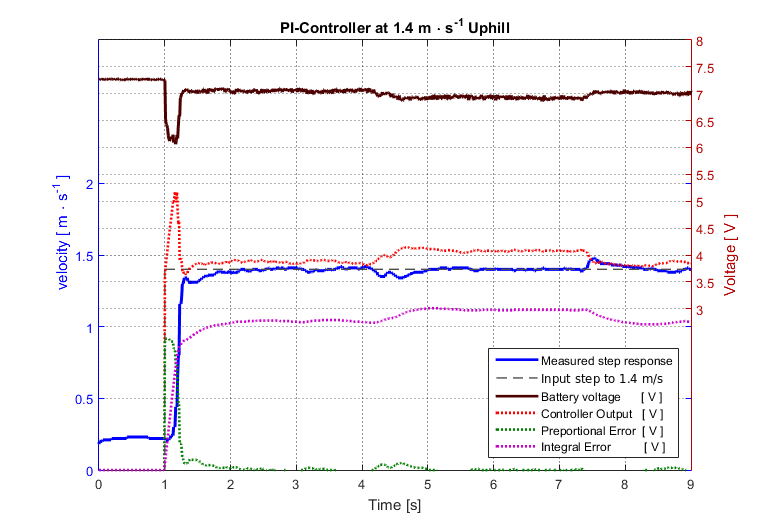
\includegraphics[scale=0.38]{Pictures/PIhill.png}   
\end{figure}

\end{frame}
%%%%%%%%%%%%%%%%

%%%%%%%%%%%%%%%%
%\subsection{PI-Controller}

% \begin{frame}{Velocity Controller}{PI-Controller}

% \begin{figure}[H]
% 	\centering
% 	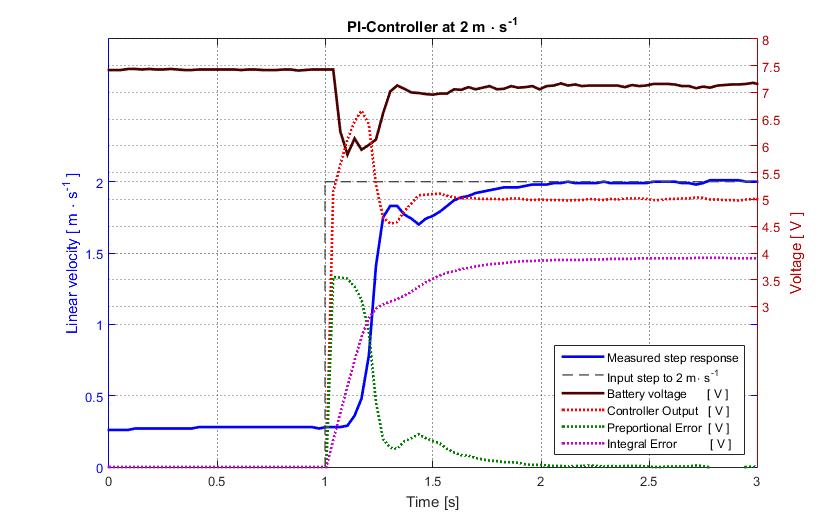
\includegraphics[scale=0.45]{Pictures/PInoAntiWindup.png}   
% \end{figure}

% \end{frame}
% %%%%%%%%%%%%%%%%

% %%%%%%%%%%%%%%%%
% %\subsection{PI-Controller}

% \begin{frame}{Velocity Controller}{PI-Controller}

% \begin{figure}[H]
% 	\centering
% 	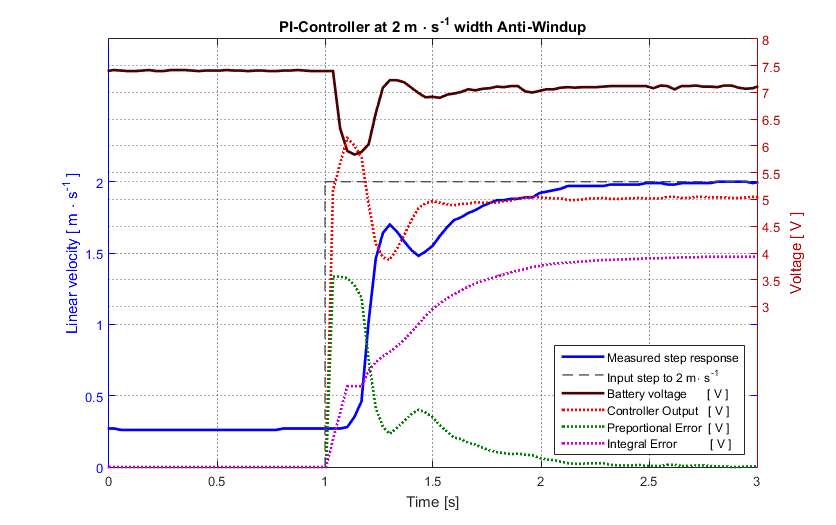
\includegraphics[scale=0.45]{Pictures/PIwidthAntiWindup.png}   
%\end{figure}

%\end{frame}
%%%%%%%%%%%%%%%%

%%%%%%%%%%%%%%%%%%%%%%%%%%% Julien %%%%%%%%%%%%%%%%%%%%%%%%%%%%%
\section{Parameters}

%- 1 -%
\begin{frame}{Model Parameters}{List of Parameters}
  \begin{table}[H]\centering
  \begin{tabular}{|c|S[table-figures-exponent=1]@{\,}|s[table-unit-alignment = left]|}
    \hline
      \textbf{Parameter}  & \multicolumn{1}{c|}{\textbf{Value}} & \multicolumn{1}{c|}{\textbf{Unit}}\\
    \hline%------------------------------------------------------------------
      \si{m_W}            & 0.222                               & \kilo\gram\\
    % \hline%------------------------------------------------------------------
      \si{l_W}            & 0.093                               & \metre\\
    % \hline%------------------------------------------------------------------
      \si{J_W}            & 0.601e-3                            & \kilo\gram\meter\squared\\
    % \hline%------------------------------------------------------------------
      \si{B_W}            & 17.03e-6                            & \newton\metre\second\per\radian\\
    % \hline%------------------------------------------------------------------
      \si{m_F}            & \multicolumn{1}{c|}{?}              & -\\
    % \hline%------------------------------------------------------------------
      \si{l_F}            & \multicolumn{1}{c|}{?}              & -\\
    % \hline%------------------------------------------------------------------
      \si{J_F}            & \multicolumn{1}{c|}{?}              & -\\
    % \hline%------------------------------------------------------------------
      \si{B_F}            & \multicolumn{1}{c|}{?}              & -\\
    \hline%------------------------------------------------------------------
  \end{tabular}
  \end{table}
\end{frame}

%- 2 -%
\subsection{Model Parameters}
\begin{frame}{Model Parameters}{Obtaining New Parameters}
  \setbeamercovered{transparent}
  \uncover<1,2>{
  \begin{itemize}
    \item Mass of the frame
  \end{itemize}
  }
  \only<2>{
    \begin{figure}[H]
      \centering
      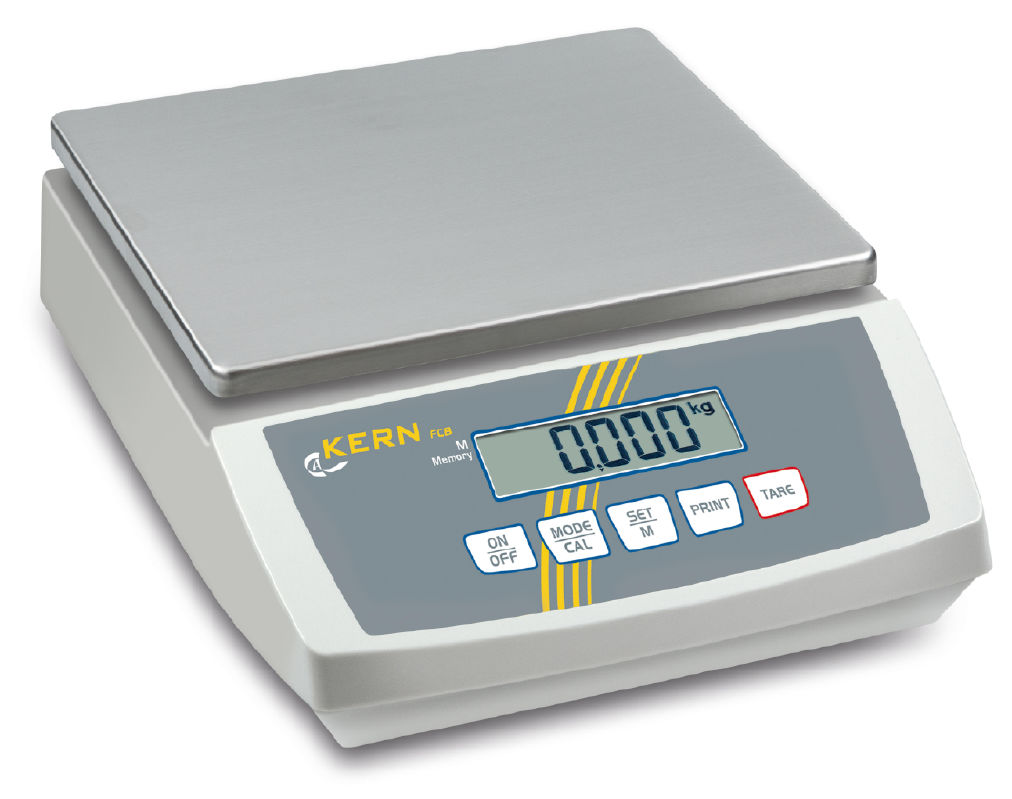
\includegraphics[scale=0.2]{Pictures/scale.jpg}
    \end{figure}
  }
  %%
  \uncover<1,3>{
  \begin{itemize}
    \item Center of mass
  \end{itemize}
  }
  \only<3>{
  \begin{figure}[H]
    \centering
    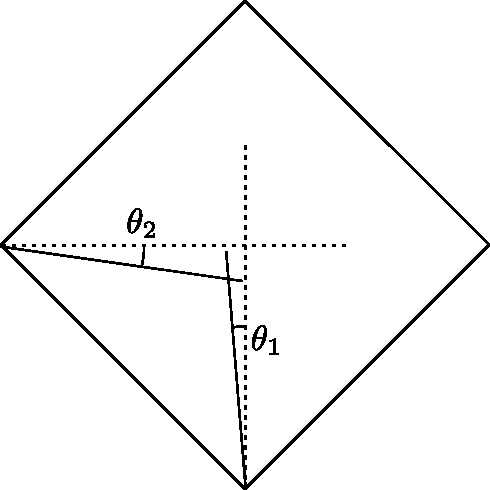
\includegraphics[scale=0.35]{Pictures/centerOfMassDiagram.pdf}
  \end{figure}
  }
  %%
  \uncover<1,4>{
  \begin{itemize}
    \item Friction and moment of inertia of the frame
  \end{itemize}
  }
  \only<4>{
    \begin{figure}[H]
    \centering
    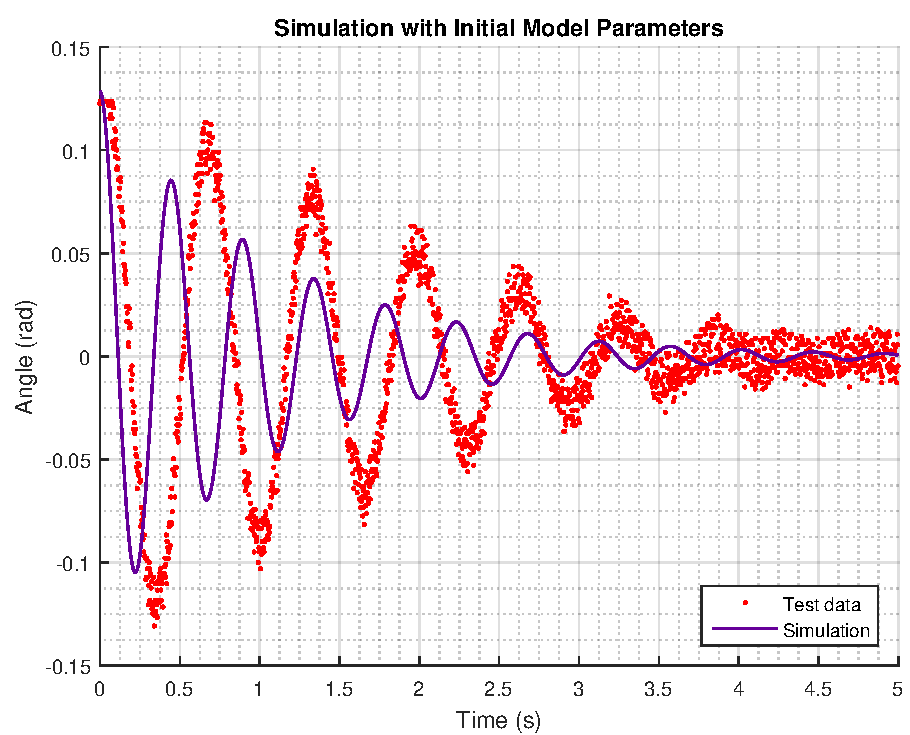
\includegraphics[scale=0.4]{Pictures/InitialModelParameterCompare.pdf}
  \end{figure}
  }
\end{frame}

%--------------------------------------------------------
\subsection{Parameter Estimation}

%- 3 -%
\begin{frame}{Parameter Estimation}{Optimization Problem}
  \begin{itemize}
    \item Optimization problem
  \end{itemize}  
  \begin{figure}[H]
      \centering
      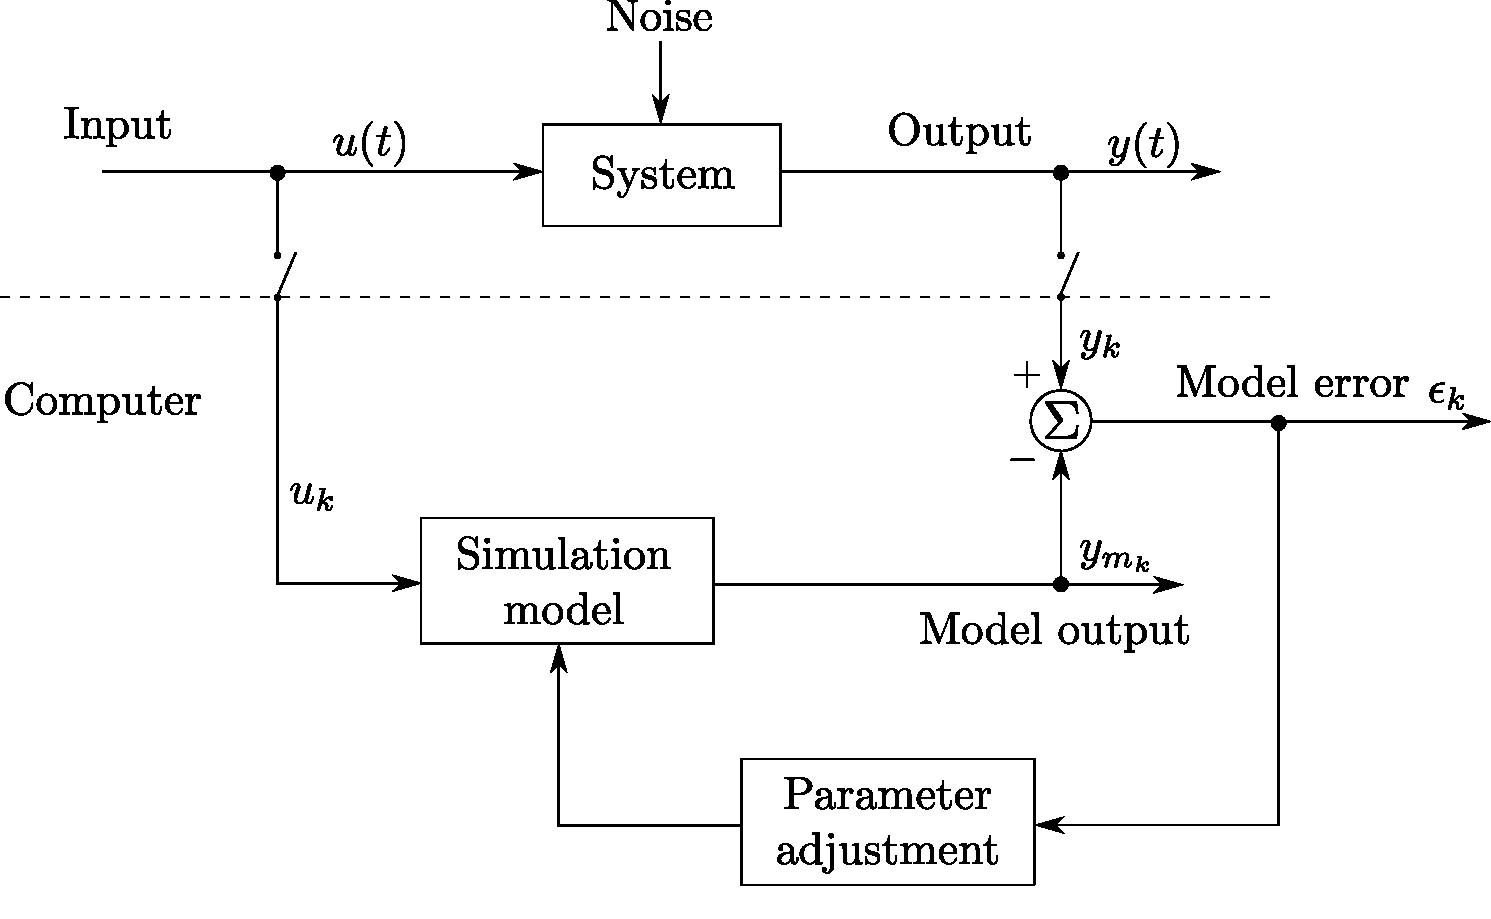
\includegraphics[scale=0.25]{Pictures/senstoolsModelOptimizationHM}
  \end{figure}\vspace{-12pt}
  \pause
  \begin{itemize}
    \item Cost function
  \end{itemize}
  \begin{displaymath}
    \si{C(\theta) = \frac{1}{2N}\sum_{k = 1}^{N} \left(y_{k} - y_{m_k}(\vec{\theta})\right)^2 }
  \end{displaymath}
\end{frame}

%- 4 -%
\begin{frame}{Parameter Estimation}{Steepest Descent (1)}
  \begin{figure}[H]
    \centering
    % (Must be redone)
    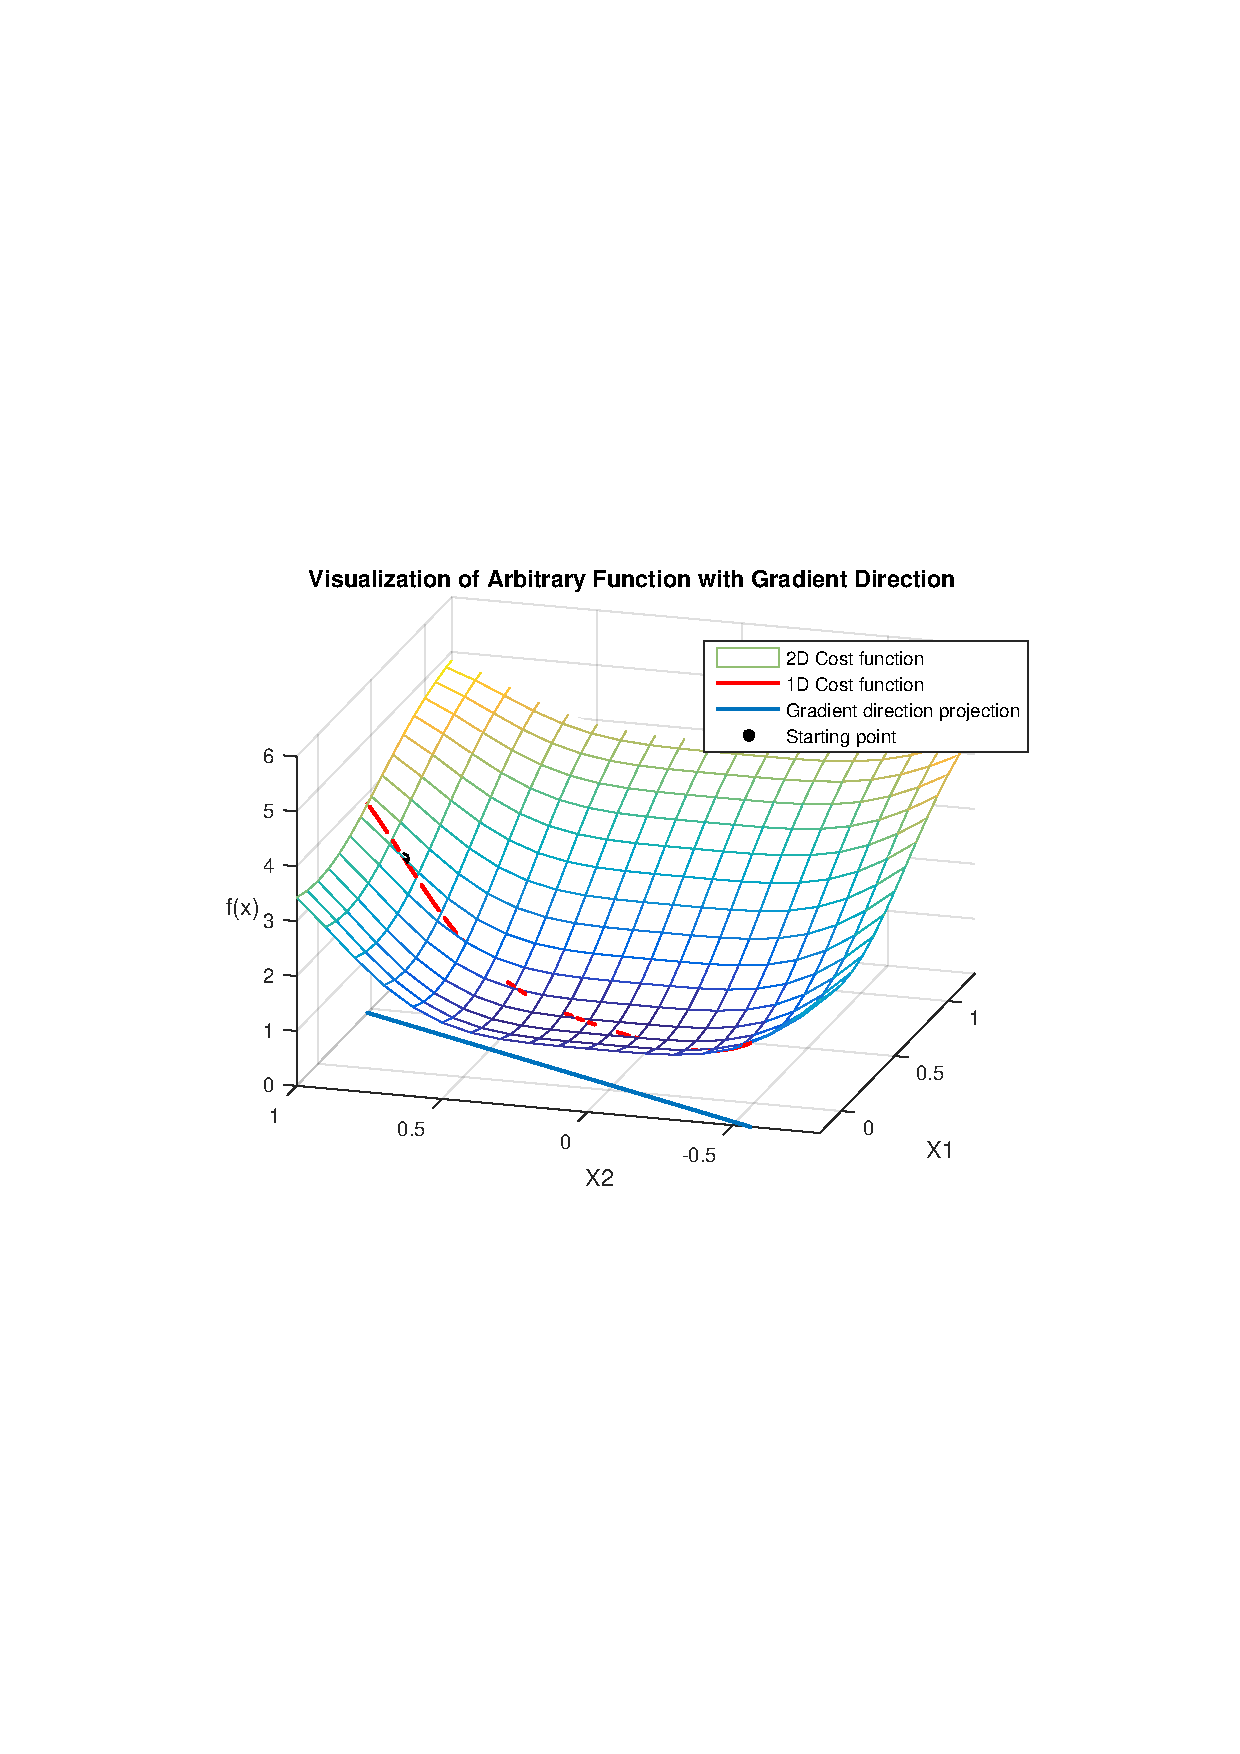
\includegraphics[scale=0.28]{Pictures/gradientDIrection2D4}
  \end{figure}
\end{frame}

\begin{frame}{Parameter Estimation}{Steepest Descent (2)}
  \begin{figure}[H]
    \centering
    % Plot of the 1D cost function along the gradient direction
    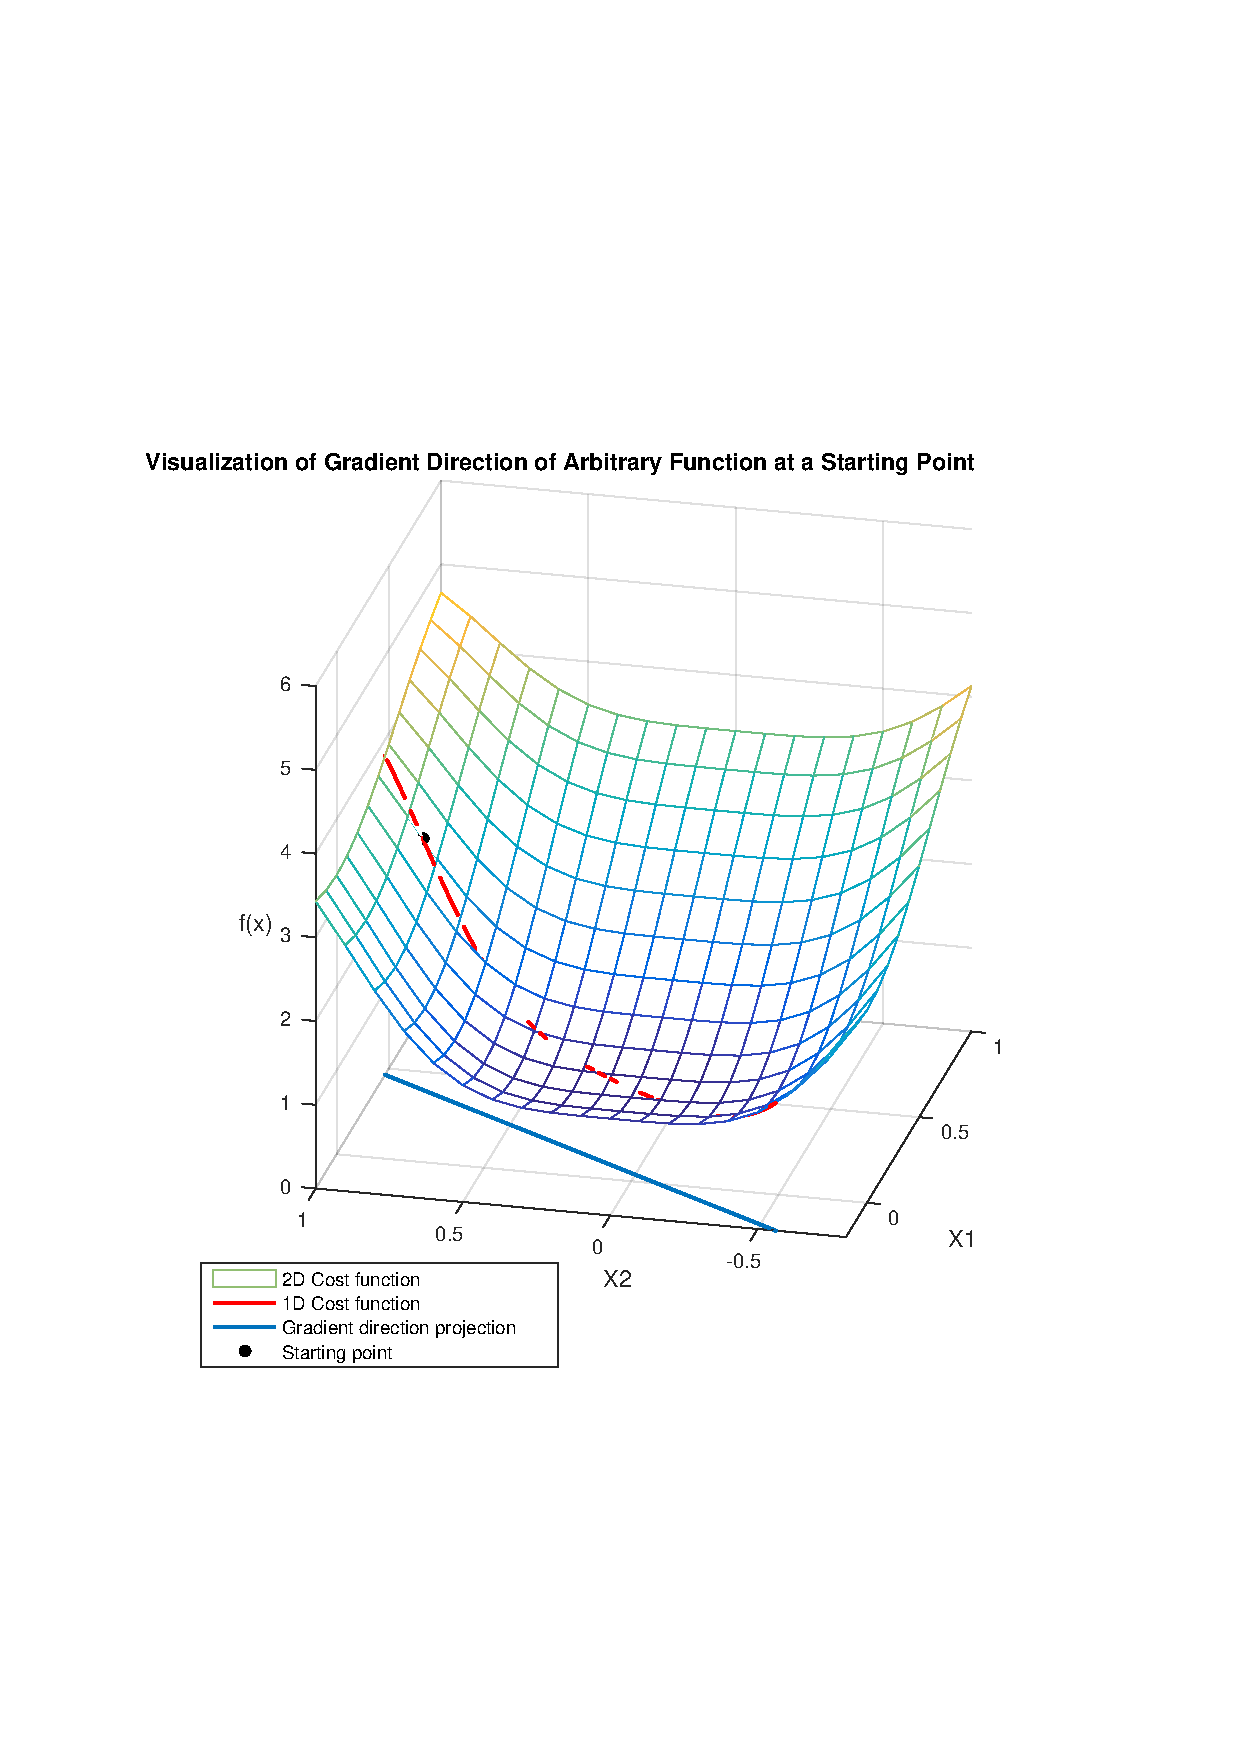
\includegraphics[scale=0.33]{Pictures/gradientDIrection1D3}
  \end{figure}
\end{frame}

%- 5 -%
\begin{frame}{Parameter Estimation}{Fibonacci Line Search}
  \begin{minipage}{\linewidth}
    \begin{minipage}{0.40\linewidth}
      \only<1>{
      \begin{figure}[H]
        \centering
        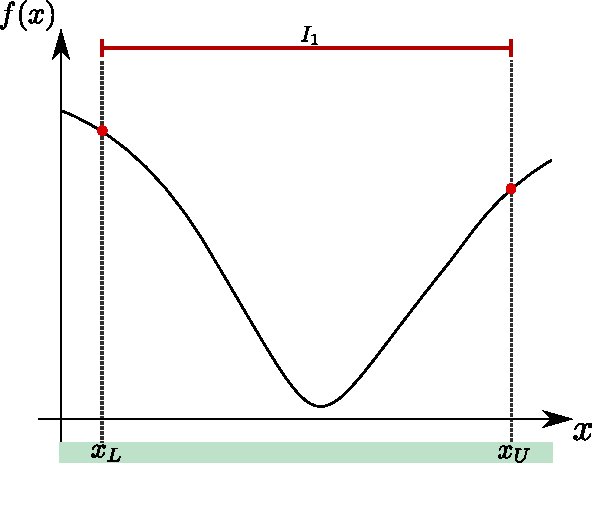
\includegraphics[scale=0.40]{Pictures/fibonacciIntervalSystem0}
      \end{figure}
      }
      \only<2>{
      \begin{figure}[H]
        \centering
        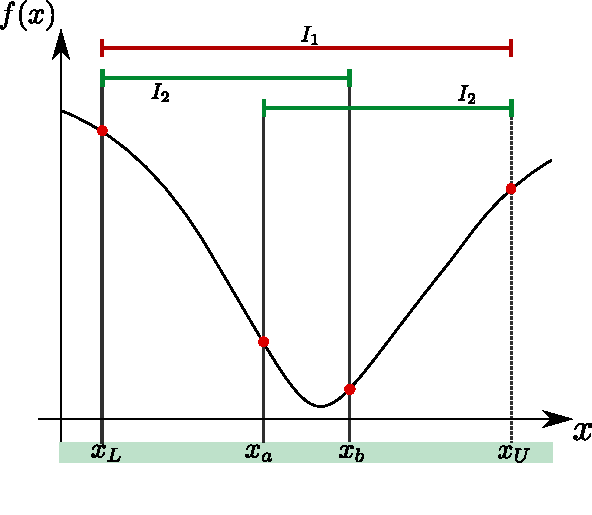
\includegraphics[scale=0.40]{Pictures/fibonacciIntervalSystem1}
      \end{figure}
      }
      \only<3>{
      \begin{figure}[H]
        \centering
        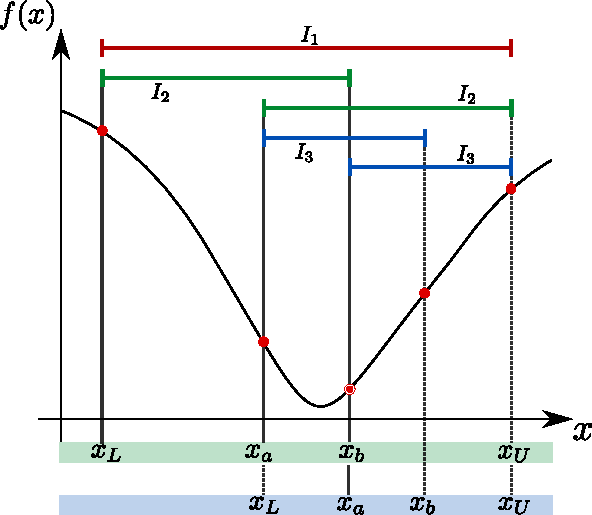
\includegraphics[scale=0.40]{Pictures/fibonacciIntervalSystem2}
      \end{figure}
      }
      \only<4->{
      \begin{figure}[H]
        \centering
        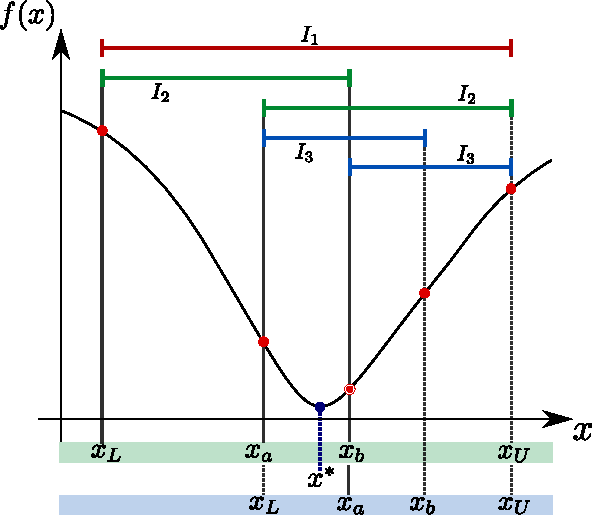
\includegraphics[scale=0.40]{Pictures/fibonacciIntervalSystem3}
      \end{figure}
      }
    \end{minipage}
    % \hspace{0.05\linewidth}
    \begin{minipage}{0.45\linewidth}
      \pause[5]
      % \only<5->{
        \begin{itemize}
          \item Initial relations
        \end{itemize}
        \begin{displaymath}
          \si{I_k = I_{k+1} + I_{k+2}, for\ all\ k=1,2,\dots,n-1}
        \end{displaymath}
        \begin{displaymath}
          \si{I_n = I_{n+1},\ assuming\ I_{n+2}=0}
        \end{displaymath}
      % }
      \vspace{-12pt}
      %%
      \pause[6]
      % \only<6>{  
        \begin{itemize}
          \item Successive relations
        \end{itemize}
        \begin{displaymath}
          \si{I_{n+1}}      =  \phantom{\si{\ I_{n+1}  + I_{n+2}         =}}\si{ 1 I_n  = F_0 I_n}
        \end{displaymath}
        \begin{displaymath}
          \si{I_{n}}\phantom{_{+1}}      =  \si{ I_{n+1}  + I_{n+2} }                    =  \si{ 1 I_n  = F_1 I_n }
        \end{displaymath}
        \begin{displaymath}
          \si{I_{n-1}}      =  \si{ I_{n} }\phantom{_{+1}} + \si{ I_{n+1} } =  \si{ 2 I_n  = F_2 I_n }
        \end{displaymath}
        \begin{displaymath}
          \vdots
          \phantom{I_{n-4}+I_{n-5}+I{4242}}
        \end{displaymath}
        \begin{displaymath}
          \si{I_{k}}\phantom{_{4}}   =  \si{ I_{k+1} + I_{k+2} = F_{n-k+1} I_n }
        \end{displaymath}
        \begin{displaymath}
          \vdots                         
          \phantom{I_{n-4}+I_{n-5}+I{4242}}
        \end{displaymath}
        \begin{displaymath}
          \si{I_{1}}\phantom{_{4}}      =  \si{ I_{2}  + I_{3} }\si{= F_n I_n }\phantom{_{k-1k+2k+3}} 
        \end{displaymath}
      % }
    \end{minipage}
  \end{minipage}
\end{frame}


%----------------------------------------------------------------
\begin{frame}{Parameter Estimation}{Forward-Backward Method}
  \begin{itemize}
    \item Goal: find an initial bracket
    \item Principle: high-low-high geometry
  \end{itemize}
  \begin{figure}[H]
    \centering
    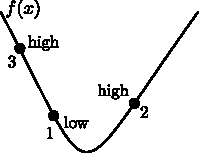
\includegraphics[scale=1.5]{Pictures/forward-backward.pdf}
  \end{figure}
\end{frame}

% \begin{frame}{Parameter Estimation}{Implementation (1)}
%   \begin{minipage}{\linewidth}\centering
%     \begin{minipage}{0.35\linewidth}
%       \begin{figure}[H]
%         \centering
%         %\transduration<0-19>{0}
%         %\multiinclude[<+->][format=png, graphics={width=\textwidth}]{Pictures/cost}
%         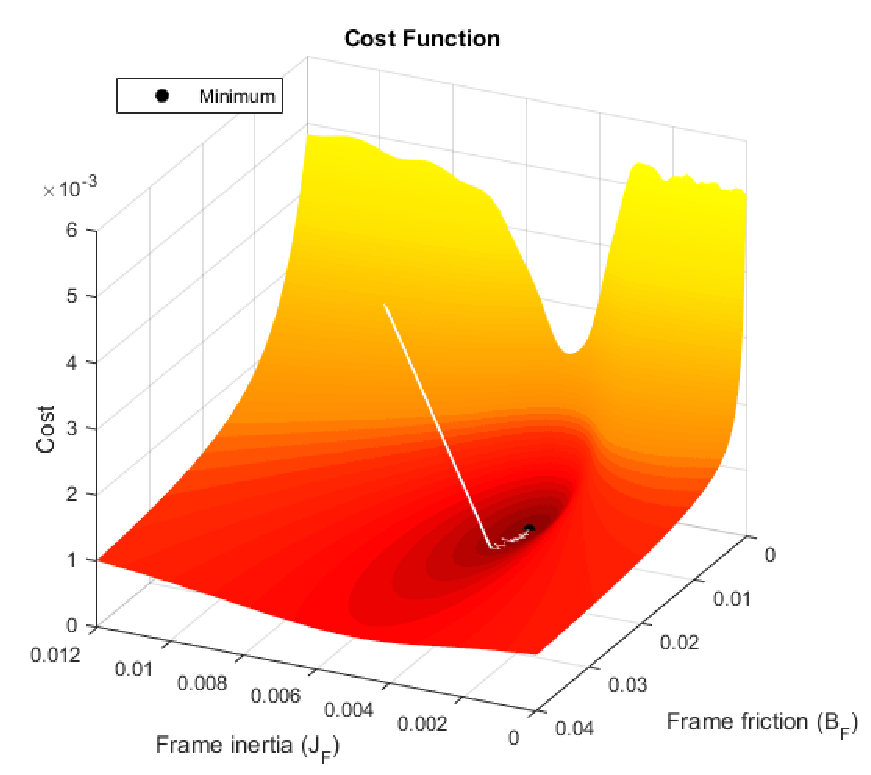
\includegraphics[scale=0.35]{Pictures/costFunctionMinimized.pdf}       
%       \end{figure}
%     \end{minipage}
%     \hspace{0.15\linewidth}
%     \begin{minipage}{0.45\linewidth}
%       \begin{figure}[H]
%         \centering
%         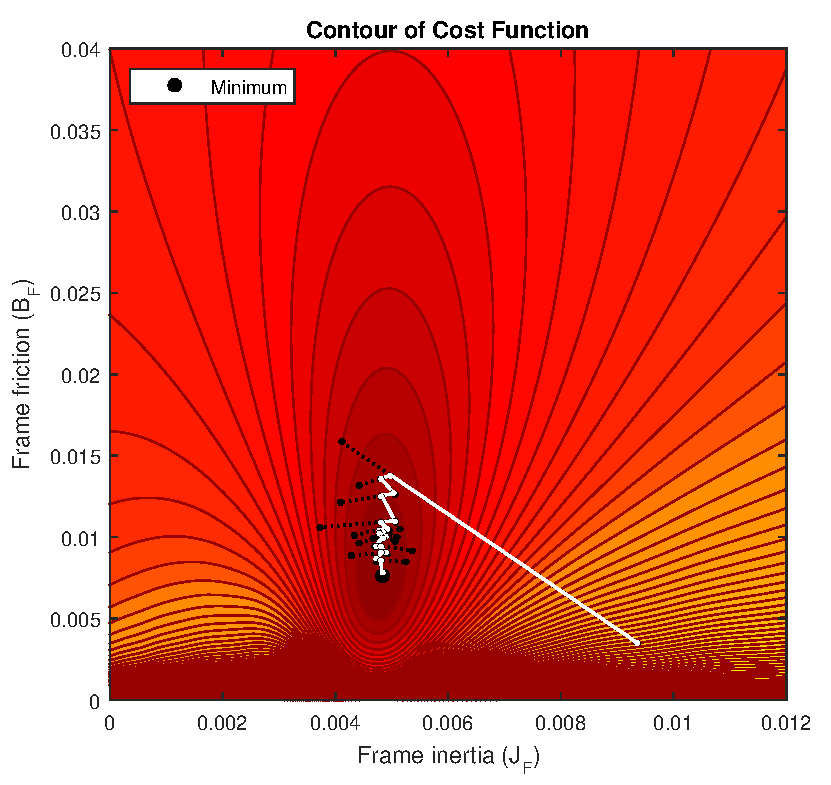
\includegraphics[scale=0.35]{Pictures/costFunctionMinimizedContour.pdf}
%       \end{figure}
%     \end{minipage}
%   \end{minipage}
%   Animated pictures would be better...
% \end{frame}

\begin{frame}{Parameter Estimation}{Implementation (1)}
  \begin{figure}[H]
    \centering
    \includegraphics[width=\textwidth]{Pictures/optJoinedFit/cost-0.png}
  \end{figure}
\end{frame}

\begin{frame}{Parameter Estimation}{Implementation (1)}
  \transduration<1-19>{0.75}
  \multiinclude[format=png, graphics={width=\textwidth}]{Pictures/optJoinedFit/cost}
  %\animategraphics[autoplay,loop,width=\linewidth]{1}{Pictures/cost-}{0}{19}
\end{frame}

\begin{frame}{Parameter Estimation}{Implementation (2)}
  \begin{minipage}{\linewidth}\centering
    \begin{minipage}{0.45\linewidth}
      \only<1->{
      \begin{figure}[H]
        \centering
        \includegraphics[scale=0.35]{Pictures/resultOfGradientWithFibonacciAndForwardBackward}
      \end{figure}
        \begin{table}[H]\centering
          \begin{tabular}{
          |c
          |S[table-figures-exponent=1,table-number-alignment=left, table-figures-integer=1]%@{\,}
          |s[table-unit-alignment = left,table-column-width=52pt]|}
            % \hline
              % \textbf{Parameter}  & \multicolumn{1}{c|}{\textbf{Value}} & \multicolumn{1}{c|}{\textbf{Unit}}\\
            \hline%------------------------------------------------------------------
              \si{J_F}            & 4.8e-3 & \kilo\gram\meter\squared         \\%& -\\
            % \hline%------------------------------------------------------------------
              \si{B_F}            & 7.8e-3 & \newton\metre\second\per\radian            \\%& -\\
            \hline%------------------------------------------------------------------
          \end{tabular}
        \end{table}
      }
    \end{minipage}
    \hspace{0.05\linewidth}
    \begin{minipage}{0.45\linewidth}
      % \only<2->{
      \pause[2]
        \begin{figure}[H]
          \centering
          \includegraphics[scale=0.35]{Pictures/SenseToolParameterEstimation}
        \end{figure}
        \begin{table}[H]\centering
          \begin{tabular}{
          |c
          |S[table-figures-exponent=1,table-number-alignment=left, table-figures-integer=1]%@{\,}
          |s[table-unit-alignment = left,table-column-width=52pt]|}
            % \hline
              % \textbf{Parameter}  & \multicolumn{1}{c|}{\textbf{Value}} & \multicolumn{1}{c|}{\textbf{Unit}}\\
            \hline%------------------------------------------------------------------
              \si{J_F}            & 4.8e-3 & \kilo\gram\meter\squared             \\%& -\\
            % \hline%------------------------------------------------------------------
              \si{B_F}            & 7.7e-3 & \newton\metre\second\per\radian            \\%& -\\
            \hline%------------------------------------------------------------------
          \end{tabular}
        \end{table}
      % }
    \end{minipage}
  \end{minipage}
\end{frame}

%------------------------------------------------------------
\subsection{Model Parameters (rev'd)}

\begin{frame}{Model Parameters}{Final Parameters}
  \begin{table}[H]\centering
  \begin{tabular}{
  |c
  |S[
    table-figures-exponent=2,
    % table-column-width=60pt
    % table-figures-integer=2,
    % table-number-alignment=right
    ]
  |s[table-unit-alignment = left]|
  }
    \hline
      \textbf{Parameter}  & \multicolumn{1}{c|}{\textbf{Value}} & \multicolumn{1}{c|}{\textbf{Unit}}\\
    \hline%------------------------------------------------------------------
      \si{m_W}            & 0.222                               & \kilo\gram\\
    % \hline%------------------------------------------------------------------
      \si{l_W}            & 0.093                               & \metre\\
    % \hline%------------------------------------------------------------------
      \si{J_W}            & 0.601e-3                            & \kilo\gram\meter\squared\\
    % \hline%------------------------------------------------------------------
      \si{B_W}            & 17.03e-6                            & \newton\metre\second\per\radian\\
    % \hline%------------------------------------------------------------------
      \si{m_F}            & 0.548                               & \kilo\gram\\
    % \hline%------------------------------------------------------------------
      \si{l_F}            & 0.08498                             & \metre\\
    % \hline%------------------------------------------------------------------
      \si{J_F}            & 4.8e-3                              & \kilo\gram\meter\squared \\
    % \hline%------------------------------------------------------------------
      \si{B_F}            & 7.7e-3                              & \newton\metre\second\per\radian\\
    \hline%------------------------------------------------------------------
  \end{tabular}
  \end{table}
\end{frame}

\section{Model Testing}
\begin{frame}{Model Testing}{Linearization of the Model}
  \begin{minipage}{\linewidth}\centering
    \begin{minipage}{0.45\linewidth}
      \begin{figure}[H]
        \centering
        \includegraphics[scale=0.33]{Pictures/LinearizedVSNonlinear}
      \end{figure}
    \end{minipage}
    % \hspace{0.05\linewidth}
    \begin{minipage}{0.45\linewidth}
      \begin{figure}[H]
        \centering
        \includegraphics[scale=0.33]{Pictures/LinearizedVSNonlinear_0}
      \end{figure}
    \end{minipage}
  \end{minipage}
\end{frame}

\begin{frame}{Model Testing}{Comparison with Real System}
  \begin{minipage}{\linewidth}\centering
    \begin{minipage}{0.45\linewidth}
      \begin{figure}[H]
        \centering
        \includegraphics[scale=0.33]{Pictures/FallTestComparison}
      \end{figure}
    \end{minipage}
    \hspace{0.03\linewidth}
    \begin{minipage}{0.45\linewidth}
      \begin{figure}[H]
        \centering
        \includegraphics[scale=0.33]{Pictures/StepTest}
      \end{figure}
    \end{minipage}
  \end{minipage}
\end{frame}
%%%%%%%%%%%%%%%%%%%%%%%%%%%%%%%%%% Niels %%%%%%%%%%%%%%%%%%%%%%%%%%%%%
%%%%%%%%%%%%%%%%%
\section{State Space}

%---------------------------------------------------------------------------------
\subsection{Motivation}%----------------------------------------------------------
%---------------------------------------------------------------------------------

\begin{frame}{State Space}{Motivation}	
  \begin{itemize}
  	\item Angular velocity of the wheel using root locus design
  \end{itemize}
  \vspace{.5cm}
  \begin{minipage}{\linewidth}
  	\begin{minipage}{0.4\linewidth}
  		\begin{figure}
  			\includegraphics[scale=.35]{Pictures/positionRLTest}
  			\centering
  		\end{figure}
  	\end{minipage}
  	\hspace{0.1\linewidth}
  	\begin{minipage}{0.45\linewidth}
  		\begin{figure}[H]
  			\includegraphics[scale=.35]{Pictures/wheelRLTest}
  			\centering
  		\end{figure}
  	\end{minipage}
  \end{minipage}
\end{frame}

\begin{frame}{State Space}{Motivation}
  \begin{itemize}
    \item Control of velocity for improved performance
    \item Classical cascade control is not feasible
  \end{itemize}
  \vspace{.2cm}
  \begin{figure}[H]
    \centering
      \begin{tikzpicture}[ auto,
                       thick,                         %<--setting line style
                       node distance=1.5cm,             %<--setting default node distance
                       scale=0.45,                     %<--|these two scale the whole thing
                       every node/.style={scale=0.50}, %<  |(always change both)
                       >/.tip={Triangle[angle=40:5pt]}
                       ]

    %-- Blocks creation --%
    \draw
      % DIRECT TERM %
      node[shape=coordinate][](input1) at (0,0){}
      node[shape=coordinate][](feedForward) at (0.5,0){}
      node(sum1) at (7.75,0) [sum] {\si{\sum}}
      node(sum2) at (9.25,0) [sum]{\si{\sum}}
      node(sum3) at (10.75,0) [sum]{\si{\sum}}

      node(torque2rotacc1) at (12.85,0) [block]{\large \si{\frac{1}{J_F + m_w \cdot {l_w}^{2}}}}

      node(integration1) at (15.75,0) [block] {\large \si{\frac{1}{s}}}
      node(integration2) at (18.2,0) [block] {\large \si{\frac{1}{s}}}

      node[shape=coordinate][](output) at (19,0){}
      node[shape=coordinate][](veloFeedbackNode) at (16.8,0){}
      node[shape=coordinate][](accFeedbackNode) at (14.5,0){}
    ;
    \draw
      % REACTION WHEEL EQUATIONS %  
      node(sum4) at (1.5,-1.6) [sum]{\si{\sum}}
      node(sum5) at (2.85,-1.6) [sum]{\si{\sum}}

      node(torque2rotacc2) at (4.3,-1.6) [block]{\large \si{\frac{1}{J_w \cdot s}}}
      % node(integration3) [block, right of = torque2rotacc2] {$\frac{1}{s}$}
      node(frictionWheel) at (6.9,-1.6) [block] {\large $B_w$}

      node[shape=coordinate][](veloWheelFeedback) at (7.75,-3.2){}
    ;
    \draw
      % FEEDBACKS %
      node(accFeedback) at (8, -4.8) [block] {\large \si{J_w}}
      node(veloFeedback) at (12.65,-1.6) [block] {\large \si{B_F}}
      node(angleFeedback) at (11.65,-3.2) [block] {\large \si{(m_F \cdot l_F + m_w \cdot l_w)g}}
    ;
    %-- Block linking --%
    % INPUT %
    \draw[-](input1)        -- node{\large \si{\tau_m(s)}}(feedForward);
    \draw[->](feedForward)  -- (sum1);

    % OUTPUT %
    \draw[-](integration2)  -- (output);
    \draw[->](output)       -- node {\large \si{\theta_{F}(s)}} (20,0);

    % DIRECT TERM %
    \draw[->] (sum1)            -- (sum2);
    \draw[->] (sum2)            -- (sum3);
    \draw[->] (sum3)            -- (torque2rotacc1);
    \draw[->] (torque2rotacc1)  -- node{\large \si{\ddot{\theta}_F(s)}}(integration1);
    \draw[->] (integration1)    -- node{\large \si{\dot{\theta}_F(s)}}(integration2);

    % REACTION WHEEL EQUATIONS %
    \draw[->] (feedForward)     |- (sum4);
    \draw[->] (sum4)            -- (sum5);
    \draw[->] (sum5)            -- (torque2rotacc2);
    \draw[->] (torque2rotacc2)  -- node{\large \si{\dot{\theta}_w(s)}}(frictionWheel);
    % \draw[->] (integration3)    -- (frictionWheel);
    \draw[->] (frictionWheel)   -| (sum1);

    \draw[-] (frictionWheel)       -| (veloWheelFeedback);
    \draw[->] (veloWheelFeedback)  -| (sum5);

    % FEEDBACKS
    \draw[->] (accFeedbackNode)  |- (accFeedback);
    \draw[->] (accFeedback)      -| (sum4);

    \draw[->] (output)           |- (angleFeedback);
    \draw[->] (angleFeedback)    -| (sum2);

    \draw[->] (veloFeedbackNode) |- (veloFeedback);
    \draw[->] (veloFeedback)     -| (sum3);

    %-- Nodes --%
    \draw%--------------------------------------------------------------
%      node at (input1)            [shift={(-0.04, -0.05 )}] {\Large \textopenbullet}
      node at (output)            [shift={( 0.007, -0.05 )}] {\Large \textbullet}
      node at (veloFeedbackNode)  [shift={( 0.007, -0.05 )}] {\Large \textbullet}
      node at (accFeedbackNode)   [shift={( 0.007, -0.05 )}] {\Large \textbullet}
      node at (feedForward)       [shift={( 0.007, -0.05 )}] {\Large \textbullet}
      node at (frictionWheel)     [shift={( 0.85, -0.04 )}] {\Large \textbullet}
    ;

    %-- Summation signs --%
      \draw%--------------------------------------------------------------
      node at (sum1) [right = -6.6mm, below = .6mm] {$-$}
      node at (sum1) [right = -3mm, below = 3.9mm]  {$+$} 
      node at (sum2) [right = -6.6mm, below = .6mm] {$+$}
      node at (sum2) [right = -3mm, below = 3.9mm]  {$+$}
      node at (sum3) [right = -6.6mm, below = .6mm] {$+$}
      node at (sum3) [right = -3mm, below = 3.9mm]  {$-$}
      node at (sum4) [right = -6.6mm, below = .6mm] {$+$}
      node at (sum4) [right = -3mm, below = 3.9mm]  {$-$}
      node at (sum5) [right = -6.6mm, below = .6mm] {$+$}
      node at (sum5) [right = -3mm, below = 3.9mm]  {$-$}
    ;

  \end{tikzpicture}
  \end{figure}
\end{frame}

%---------------------------------------------------------------------------------
\subsection{Model}%---------------------------------------------------------------
%---------------------------------------------------------------------------------

\begin{frame}{State Space}{Model}

  \begin{itemize}
  	\item State, output and input variables
  \end{itemize}

  \begin{minipage}{0.29\linewidth}
       	\begin{flalign}
       		\vec{x} = 
       		\begin{bmatrix}
       			\theta_F \\
       			\dot{\theta}_F \\ 
       			\dot{\theta}_w \\
       		\end{bmatrix}\nonumber
       	\end{flalign}  
      \end{minipage}
      %\hspace{0.03\linewidth}
      \begin{minipage}{0.29\linewidth}
       	\begin{flalign}
       		\vec{y} = 
       		\begin{bmatrix}
       			\theta_F \\
       			\dot{\theta}_w \\
       		\end{bmatrix}\nonumber
       	\end{flalign}
      \end{minipage}
      %\hspace{0.03\linewidth}
      \begin{minipage}{0.29\linewidth}
       	\begin{flalign}
       		\vec{u}= 
       		\begin{bmatrix}
       			\tau_m\\
       		\end{bmatrix}	\nonumber
       	\end{flalign}
    \end{minipage}
  \vspace{.5cm}
  \begin{itemize}
  	\item System of differential equations
  \end{itemize}
  %
  \begin{flalign}
  	&\hspace{.85cm} \si{\vec{\dot{x}} = f(\vec{x},\vec{u})}& \nonumber \\
  	&\hspace{.85cm} \si{\vec{y} = g(\vec{x})}& \nonumber
  \end{flalign}
\end{frame}

\begin{frame}{State Space}{Model}

  \only<1-2>
  {
    \tikz[overlay,xshift=4.5em,yshift=10ex]{\draw node {
      \begin{minipage}{0.01\linewidth}
      	  \begin{flalign}
        	  	& \hspace{1 cm} \si{\vec{\dot{x}}(t) =\ } \si{ \vec{A} \cdot \vec{x}(t) + \vec{B} \cdot \vec{u}(t)} \nonumber \\
        	  	& \hspace{1 cm} \si{\vec{y}(t) =\ } \si{ \vec{C} \cdot \vec{x}(t) } \nonumber
      	  \end{flalign}
      \end{minipage}
      \begin{minipage}{0.01\linewidth}
        \begin{tabular}{ p{.1cm} l l l}
          &&\\
          	& \si{\vec{A}=\frac{\partial}{\partial \vec{x}} \ f(\vec{x_o},\vec{u_o})}			& state     \\                       
          	& \si{\vec{B}=\frac{\partial}{\partial \vec{u}} \ f(\vec{x_o},\vec{u_o})}			& input     \\ 
          	& \si{\vec{C}=\frac{\partial}{\partial \vec{x}} \ g(\vec{x_o})}			& output
        \end{tabular} 
      \end{minipage}
    };}
  }
  
  \only<1>
  {
  \begin{textblock*}{15cm}(3cm,5.25cm)
    \tikz[overlay,xshift=9.5em,yshift=3ex]{\draw node [fontscale=\footnotesize]{
                \si{\ddot{\theta}_F = -\frac{B_F}{J_F + m_w \cdot {l_w}^2} \cdot \dot{\theta}_F + \frac{(m_F \cdot l_F + m_w \cdot l_w) \cdot g}{J_F + m_w \cdot {l_w}^2} \cdot \theta_F}
                };}
    \tikz[overlay,xshift=9.5em,yshift=-0.7ex]{\draw node [fontscale=\footnotesize]{
                 \si{- \frac{1}{J_F + m_w \cdot {l_w}^2} \cdot \tau_m + \frac{B_w}{J_F + m_w \cdot {l_w}^2} \cdot \dot{\theta}_w}
                 };}
    \tikz[overlay,xshift=10.2em,yshift=-6ex]{\draw node [fontscale=\footnotesize]{
                  \si{\ddot{\theta}_w = \frac{J_w+J_F+m_w \cdot {l_w}^{2}}{J_w \cdot (J_F+m_w \cdot {l_w}^{2})} \cdot \tau_m - \frac{(J_w+J_F+{l_w}^{2} \cdot m_w) \cdot B_w}{J_w \cdot (J_F+m_w \cdot  {l_w}^2)} \cdot \dot{\theta}_w}
                };}
    \tikz[overlay,xshift=9.7em,yshift=-10ex]{\draw node [fontscale=\footnotesize]{
                  \si{- \frac{(m_F \cdot l_F + m_w \cdot l_w) \cdot g}{J_F+m_w \cdot {l_w}^{2}} \cdot \theta_F + \frac{B_F}{J_F+m_w \cdot {l_w}^{2}} \cdot \dot{\theta}_F}
             };}
  \end{textblock*}
  }
  
  \only<2>
  {
    \begin{textblock*}{15cm}(3cm,5cm)
    	\begin{tikzpicture}[ auto,
                       thick,                         %<--setting line style
                       node distance=1.5cm,             %<--setting default node distance
                       scale=.9,                     %<--|these two scale the whole thing
                       every node/.style={scale=.9}, %<  |(always change both)
                       >=triangle 45 ]                %<--sets the arrowtype
    
    \draw%-----------------------------------------------------------------------------------------
    	%Drawing Input/Output:
    	node[shape=coordinate][](input1) at (0,0){}
    	node[shape=coordinate][](output1) at (8,0){}
     	%Drawing the Equation Blocks:   	
      	node(A) at (4.5,-1.5) [block] {A} 
     	node(B) at (1.5,0) [block] {B}
     	node(C) at (6.5,0) [block] {C}
%      	node(D) at (4.5,1.5) [block] {D}  
	    node(int) at (4.5,0) [block] {\si{\int}}  
    	%Drawing the Sumation Blocks:	    	 	
    	node(sum1) [sum, right of = B] {\si{\sum}}
%    	node(sum2) [sum, right of = C] {\si{\sum}}
    	%Drawing the Feedback/Feedforward Nodes:    	
    	node[shape=coordinate][](FeedforwardNode) at (0.75,0){}
    	node[shape=coordinate][](FeedbackNode) at (5.5,0){}  	
    	     
    ;%---------------------------------------------------------------------------------------------
   
    %Joining the Blocks
  	\draw[->](input1) -- node {u}(B);
  	\draw[->](B) -- node {}(sum1);
  	\draw[->](sum1) -- node {\si{\dot x}}(int);  	
  	\draw[->](int) -- node {x}(C);
  	\draw[->](C) -- node {y}(output1);
  	
%  	\draw[->](FeedforwardNode) |- node{} (D);
%  	\draw[->](D) -| node{} (sum2);

  	\draw[-] (FeedbackNode) |- (A);
  	\draw[->] (A)   -| (sum1);

    %Drawing node(s) with \textbullet
    \draw%--------------------------------------------------------------
%      node at (input1)  [shift={(-0.04, -0.04 )}] {\large \textbullet}
    	% node at (output1) [shift={( 0.008, -0.02 )}] {\textbullet}
    ;%------------------------------------------------------------------
  \end{tikzpicture}
  	\end{textblock*}
  }
  \only<1-2>
    {
    \tikz[overlay,xshift=7.5em,yshift=-16ex]{\draw node {
        \begin{minipage}{0.01\linewidth}
         	\begin{flalign}
         		\vec{x} = 
         		\begin{bmatrix}
         			\theta_F \\
         			\dot{\theta}_F \\ 
         			\dot{\theta}_w \\
         		\end{bmatrix}	\textbf{,}\ \nonumber
         	\end{flalign}  
        \end{minipage}
        %\hspace{0.03\linewidth}
        \begin{minipage}{0.01\linewidth}
         	\begin{flalign}
         		\vec{y} = 
         		\begin{bmatrix}
         			\theta_F \\
         			\dot{\theta}_w \\
         		\end{bmatrix}	\textbf{,}\ \nonumber
         	\end{flalign}
        \end{minipage}
        %\hspace{0.03\linewidth}
        \begin{minipage}{0.01\linewidth}
         	\begin{flalign}
         		\vec{u}= 
         		\begin{bmatrix}
         			\tau_m\\
         		\end{bmatrix}	\nonumber
         	\end{flalign}
      \end{minipage}
    };}
  }   
\end{frame}

%---------------------------------------------------------------------------------
\subsection{Controller Design}%---------------------------------------------------
%---------------------------------------------------------------------------------
\begin{frame}{State Space}{Controller Design}
  \begin{itemize}
    \item Eigenvalues of \si{(\vec{A} - \vec{B} \vec{K})}
    \item Pole placement
  \end{itemize}

  \begin{displaymath}
  	\hspace{-5cm}\si{\vec{\dot{x}}(\vec{t}) = (\vec{A}-\vec{B}\vec{K}) \cdot \vec{x}(\vec{t})} \nonumber
  \end{displaymath}
  
  \begin{figure}[H]
      \centering
      \begin{tikzpicture}[ auto,
					thick,                         %<--setting line style
					node distance=1.5cm,             %<--setting default node distance
					scale=1,                     %<--|these two scale the whole thing
					every node/.style={scale=1}, %<  |(always change both)
					>=triangle 45 ]                %<--sets the arrowtype

	\draw%-----------------------------------------------------------------------------------------
	%Drawing Input/Output:
	node[shape=coordinate][](input1) at (0,0){}
	node[shape=coordinate][](inputFeedback) at (.3,0){}
	node[shape=coordinate][](output1) at (8,0){}
	%Drawing the Equation Blocks:   	
	node(A) at (4,-1.5) [block] {A} 
	node(B) at (1.5,0) [block] {B}
	node(C) at (6.5,0) [block] {C}
	node(int) at (4.5,0) [block] {\si{\int}} 
	node(K) at (2.8,-2.5) [block] {-K}	
	%Drawing the Sumation Blocks:	    	 	
	node(sum1) [sum, right of = B] {\si{\sum}}
	%Drawing the Feedback/Feedforward Nodes:    	
	node[shape=coordinate][](FeedbackNode) at (5.2,0){}  	
	node[shape=coordinate][](FeedbackNode2) at (5.6,0){} 
	
	;%---------------------------------------------------------------------------------------------

	%Joining the Blocks
	\draw[->](input1) -- node {u}(B);
	\draw[->](B) -- node {}(sum1);
	\draw[->](sum1) -- node {\si{\dot x}}(int);  	
	\draw[->](int) -- node {x}(C);
	\draw[->](C) -- node {y}(output1);

	\draw[->] (FeedbackNode) |- (A);
	\draw[->] (A)   -| (sum1);
	
	\draw[->] (FeedbackNode2) |- (K);
	\draw[-] (K)   -| (inputFeedback);

	%Drawing node(s) with \textbullet
	\draw%--------------------------------------------------------------
%	node at (input1)  [shift={(-0.08, -0.02 )}] {\large \textbullet}
	% node at (output1) [shift={( 0.008, -0.04 )}] {\textbullet}
	;%------------------------------------------------------------------

\end{tikzpicture}
  \end{figure}
\end{frame}

\begin{frame}{State Space}{Controller Design}
  \begin{itemize}
    \item Controller reacting to disturbance
    \item Different pole placements
    \item The yellow was chosen
  \end{itemize}
  \vspace{.5cm}
  \hspace{0.03\linewidth}
  \begin{minipage}{\linewidth}
   	\begin{minipage}{0.45\linewidth}
   		\begin{figure}[H]
   			\includegraphics[scale=.35]{Pictures/disturbanceStateSpace}
   			\centering
   		\end{figure}
   	\end{minipage}
   	\hspace{0.03\linewidth}
   	\begin{minipage}{0.45\linewidth}
   		\begin{figure}[H]
   			\includegraphics[scale=.35]{Pictures/disturbanceStateSpaceWheel}
   			\centering
   		\end{figure}
   	\end{minipage}
  \end{minipage}
\end{frame}

%---------------------------------------------------------------------------------
\subsection{Controller Analysis}%-------------------------------------------------
%---------------------------------------------------------------------------------

\begin{frame}{State Space}{Controller Analysis}
    \begin{minipage}{\linewidth}
    	\begin{minipage}{0.4\linewidth}
    		\begin{figure}
    			\includegraphics[scale=.35]{Pictures/positionRLTest}
    			\centering
    		\end{figure}
    	\end{minipage}
    	\hspace{0.1\linewidth}
    	\begin{minipage}{0.45\linewidth}
    		\begin{figure}[H]
    			\includegraphics[scale=.35]{Pictures/wheelRLTest}
    			\centering
    		\end{figure}
    	\end{minipage}
    \end{minipage}
  \vspace{.5cm}
  \begin{minipage}{\linewidth}
   	\begin{minipage}{0.45\linewidth}
   		\begin{figure}[H]
   			\includegraphics[scale=.35]{Pictures/positionSSTest}
   			\centering
   		\end{figure}
   	\end{minipage}
   	\hspace{0.03\linewidth}
   	\begin{minipage}{0.45\linewidth}
   		\begin{figure}[H]
   			\includegraphics[scale=.35]{Pictures/wheelSSTest}
   			\centering
   		\end{figure}
   	\end{minipage}
  \end{minipage}
\end{frame}


% %---------------------------------------------------------------------------------
% \subsection{Animation Test}%------------------------------------------------------
% %---------------------------------------------------------------------------------

% \begin{frame}{Animation Test}{wooohooo}
%   \transduration<0-19>{1.5}
%   \multiinclude[format=png, graphics={width=\textwidth}]{Pictures/optJoinedFit/cost}
%   %\animategraphics[autoplay,loop,width=\linewidth]{1}{Pictures/cost-}{0}{19}
% \end{frame}
%%%%%%%%%%%%%%%%%%%%%%%%%%%%%%%%%% NAME %%%%%%%%%%%%%%%%%%%%%%%%%%%%%
%%%%%%%%%%%%%%%%%

\section{Acceptance Test}

%%%%%%%%%%%%%%%%% BEGIN ACCEPTANCE TEST  %%%%%%%%%%%%%%%
%%%%%%%%%%%%%Frame 1 %%%%%%%

\begin{frame}{Acceptance Test}{Requirement 1}

\begin{table}[H] \centering
\begin{tabular}{|p{0.5cm}| p{7cm} |p{1cm}|}
\hline%
\textbf{No.}  &  \textbf{Requirement}  & \textbf{Done?}     \\ 
\hline
1 & It shall be possible for the vehicle to receive its own location wirelessly from the GoT system, through a computer. & Yes \\
\hline
\end{tabular}
\end{table}

  \pause

%%% Test  %%%
\begin{table}[H]
\centering
\begin{tabular}{|l|l|l|}
\hline
GoT log file & Arduino received & Equal? \\
\hline
53,-23,-271 & 53,-23,-271 & Yes \\
\hline
53,-24,-264 & 53,-24,-264 & Yes \\
\hline
53,-24,-269 & 53,-24,-269 & Yes \\
\hline
55,-24,-267 & 55,-24,-267 & Yes \\
\hline
55,-23,-269 & 55,-23,-269 & Yes \\
\hline
56,-23,-274 & 56,-23,-274 & Yes \\
\hline
57,-22,-274 & 57,-22,-274 & Yes \\
\hline
59,-21,-274 & 59,-21,-274 & Yes \\
\hline
57,-22,-270 & 57,-22,-270 & Yes \\
\hline
55,-23,-269 & 55,-23,-269 & Yes \\
\hline
\end{tabular}
\end{table}

\end{frame}


%%%%%%%%%%%%%%%%% Frame 2 %%%%%%%%%%%


\begin{frame}{Acceptance Test}{Requirement 2}

\begin{table}[H] \centering
\begin{tabular}{|p{0.5cm}| p{7cm} |p{1cm}|}
\hline%
\textbf{No.}  &  \textbf{Requirements}    & \textbf{Done?}     \\ 
\hline
2 & It shall be possible for the prototype to disregard incorrect packets transmitted from the computer. & Yes \\ 
\hline
\end{tabular}
\end{table}

  \pause

%%% Test 2 %%%
\begin{table}[H]
\centering
\begin{tabular}{|p{2cm}|p{3cm}|p{2cm}|}
\hline
Package & Error & Error value \\
\hline
1 & No error & 0 \\
\hline
2 & Wrong start byte & 1 \\
\hline
3 & No error & 0 \\
\hline
4 & Checksum fail & 4 \\
\hline
5 & Wrong ID & 2 \\
\hline
\end{tabular}
\end{table}

\end{frame}

%%%%%%%%%%%%%%%% frame 3 %%%%%%%%%%%%


\begin{frame}{Acceptance Test}{Requirement 3}

\begin{table}[H] \centering
\begin{tabular}{|p{0.5cm}| p{7cm} |p{1cm}|}
\hline
\textbf{No.}  &  \textbf{Requirements} & \textbf{Done?}     \\ 
\hline
3 & The prototype must be able to disregard erroneous coordinates sent from the GoT system. & Yes \\ \hline
\end{tabular}
\end{table}

  \pause

%%% Test 3 %%%
\begin{figure}[H]
  \centering
  \includegraphics[scale=0.4]{Pictures/plot3.pdf}
\end{figure}

\end{frame}

%%%%%%%%%%%%%%% frame 4 %%%%%%%%%%%%%%%%%%%%


\begin{frame}{Acceptance Test}{Requirement 4}

\begin{table}[H] \centering
\begin{tabular}{|p{0.5cm}| p{7cm} |p{1cm}|}
\hline
\textbf{No.}  &  \textbf{Requirements} & \textbf{Done?}     \\ 
\hline
4 & The prototype must be able to access the route, which it has to follow, from a storage space located on the vehicle. & No \\ 
\hline
\end{tabular}
\end{table}
\end{frame}

%%%%%%%%%%%%%%%% frame 5 %%%%%%%%%%%%%%


\begin{frame}{Acceptance Test}{Requirement 5}

\begin{table}[H] \centering
\begin{tabular}{|p{0.5cm}| p{7cm} |p{1cm}|}
\hline
\textbf{No.}  &  \textbf{Requirements} & \textbf{Done?}     \\ 
\hline
5 & The prototype must be able to shut down, if the battery voltage is below its 
cut-off specification. & Yes \\ 
\hline
\end{tabular}
\end{table}
\end{frame}

%%%%%%%%%%%%%%%% frame 6 %%%%%%%%%%%%%%%%


\begin{frame}{Acceptance Test}{Requirement 6}

\begin{table}[H] \centering
\begin{tabular}{|p{0.5cm}| p{7cm} |p{1cm}|}
\hline
\textbf{No.}  &  \textbf{Requirements} & \textbf{Done?}     \\ 
\hline
6 & It shall be possible for the prototype to follow a predetermined route.  & No \\ \hline
\end{tabular}
\end{table}

  \pause

%%% Test 6 %%%
\begin{figure}[H]
  \centering
	\includegraphics[scale=0.5]{Pictures/AccTest6.pdf}
\end{figure}
\end{frame}

%%%%%%%%%%%%%%%% frame 7 %%%%%%%%%%%%

\begin{frame}{Acceptance Test}{Requirement 7}

\begin{table}[H] \centering
\begin{tabular}{|p{0.5cm}| p{7cm} |p{1cm}|}
\hline%
\textbf{No.}  &  \textbf{Requirements} & \textbf{Done?}     \\ 
\hline%
7 & It shall be possible for the prototype to return to the predetermined route if disturbed.  & No \\ \hline
\end{tabular}
\end{table}

  \pause

%%% Test 7 %%%
\begin{figure}[H]
  \centering
	\includegraphics[scale=0.5]{Pictures/AccTest7.pdf}
\end{figure}


\end{frame}

%%%%%%%%%%%%%%%% frame 8 %%%%%%%%%%%%%%%


\begin{frame}{Acceptance Test}{Requirement 8}

\begin{table}[H] \centering
\begin{tabular}{|p{0.5cm}| p{7cm} |p{1cm}|}
\hline%
\textbf{No.}  &  \textbf{Requirements} & \textbf{Done?}     \\ 
\hline%
8 & The prototype shall be able to keep a velocity on 1,4 $m \cdot s^{-1}$, when going up or downhill and when turning.  & Yes \\ \hline
\end{tabular}
\end{table}

  \pause


  \begin{minipage}{\linewidth}
  	\begin{minipage}{0.45\linewidth}
  		\begin{figure}[H]
  			\includegraphics[scale=0.38]{Pictures/AccTest8U.png}
  			\centering
  			%\vspace{-.4cm}
  		\end{figure}
  	\end{minipage}
  	\hspace{0.03\linewidth}
  	\begin{minipage}{0.45\linewidth}
  		\begin{figure}[H]
  			\includegraphics[scale=.38]{Pictures/AccTest8D.png}
  			\centering
  			%\vspace{-.4cm}
  		\end{figure}
  	\end{minipage}
  \end{minipage}

\end{frame}

%%%%%%%%%%%%%%%% END ACCEPTANCE TEST %%%%%%%%%%%%%%%



%%%%%%%%%%%%%%%%BEGIN CONCLUSION %%%%%%%%%%%%%%%
\subsection{Conclusion}

\begin{frame}{Conclusion}{What has been done?}

\pause

  \begin{itemize}
    \item<1-> Alternative navigation approaches with Games on Track system
    \item<2-> Belt vehicle analized to build prototype requirements
    \item<3-> Real Time Operating System implemented on the Arduino Mega
    \item<4-> XBee modules with protocol error handling
    \item<5-> Digital filter to lower the noise
    \item<6-> SD card storage
    \item<7-> Mathematical models simulated
    \item<8-> Distance model tests
    \item<9-> P and PI Controllers tested
  \end{itemize}
\end{frame}

%%%%%%%%%%%%%%%%END CONCLUSION %%%%%%%%%%%%%%%



%%%%%%%%%%%%%%%% BEGIN DISCUSSION %%%%%%%%%%
\subsection{Discussion}

\begin{frame}{Discussion}{What next?}

\pause

  \begin{block}{Functionalities missing from the requirements}
  	  The  steering controller could not be tested, because of magnetometer indoor disturbances.\\
      The non-volatile storage could be solved with more time.
  \end{block}
  
  \pause
  
  \textbf{What could we improve on this project?}
   \begin{itemize}
    \item<1-> The belt vehicle, not enough control
    \pause
    \item<2-> The GoT system, good accuracy but not large range
    \item<3-> Route planning and initial mapping
    \item<4-> Blade control
    \item<5-> Other functionalities (humidity, obstacle, or length detection) 
    \end{itemize}
\end{frame}
%%%%%%%%%%%%%%%% END DISCUSSION %%%%%%%%%%%%%









\end{document}
